% !TEX program = lualatex
\documentclass[12pt, openany]{book}

\usepackage[
  paperwidth=188mm,
  paperheight=263mm,
  top=18mm, bottom=18mm,
  inner=18mm, outer=18mm,
  includehead=false, includefoot=false
]{geometry}

\usepackage{luatexja-fontspec}
\setmainfont{Harano Aji Mincho}
\setsansfont{Harano Aji Gothic}
\setmainjfont{Harano Aji Mincho}
\setsansjfont{Harano Aji Gothic}

\usepackage{fontspec}
\usepackage{amsmath,amssymb}
\usepackage{unicode-math}
\usepackage{graphicx}
\usepackage{enumerate}
\usepackage{subcaption}
\usepackage{bm}


% \usepackage{here}
\usepackage{luatexja}
% \setmathfont{LatinModernMath-Regular}
\setmathfont{Latin Modern Math}
% \usepackage{booktabs}

% \usepackage{physics2}

\usepackage{tikz}
\usetikzlibrary{circuits.logic.US, positioning}
% \usepackage{circuitikz}
% \usepackage{wrapfig}
% \usepackage{float}
% \usepackage{fancyhdr}
% \pagestyle{fancy}
% \fancyhf{}
% \fancyhead[LE,RO]{\thepage}
% \fancyhead[LO,RE]{\leftmark}
\usepackage{pxrubrica}


\usepackage[hidelinks]{hyperref}

\renewcommand{\figurename}{図}
\renewcommand{\tablename}{表}
% Chapter を「第○章」にする
\renewcommand{\chaptername}{第}
\renewcommand{\thechapter}{\arabic{chapter}}

% ヘッダ（右上の Chapter ○）の修正
\renewcommand{\chaptermark}[1]{%
  \markboth{第\thechapter 章\ #1}{}%
}

\makeatletter
\renewcommand{\@makechapterhead}[1]{%
  \vspace*{50\p@}%
  {\parindent \z@ \raggedright \normalfont
    \Huge\bfseries
    \chaptername\thechapter 章\quad #1\par\nobreak
    \vskip 40\p@
  }}
\makeatother

% 目次のタイトルの修正
\renewcommand{\contentsname}{目次}

\pagestyle{plain}



\begin{document}


% --- 表紙 ---
% \vspace{\fill}
% \begin{center}
%   {\Large サークル名: ありさん工房}\\[2em]
%   {\LARGE タイトル: 論理回路入門}\\[2em]
%   {\large 著者:fry , yt}\\[1em]
%   {\small 発行日: 2025年12月31日}
% \end{center}
% \begin{figure}[htbp]
%   \centering
%   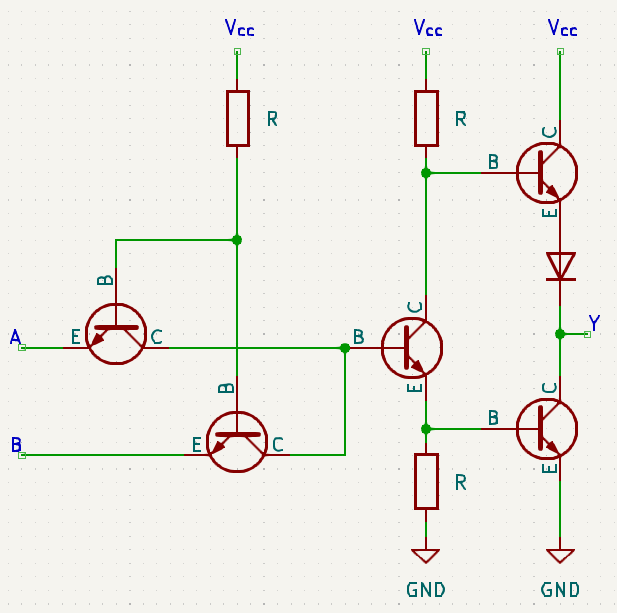
\includegraphics[width=0.9\textwidth]{BJT_logic/ttl_totem_pole.png}
% \end{figure}
% \newpage

% ---表紙裏---
% --- 目次 ---
\tableofcontents
\newpage

% --- 本文 ---
%はじめに
\chapter{はじめに}
論理回路とは、今現在、我々の生活に欠かせないものとなっている。
具体的には、コンピュータやスマートフォン、家電製品、自動車など、様々な電子機器に組み込まれている。
読者の生活にも必要不可欠なものであると言えるだろう。
しかし、もし、論理回路のない無人島に一人で投げ出されてしまった場合、論理回路の作り方を知らなければ、論理回路を作ることができず
、生活に必要な電子機器を自作することができずに野垂死にしてしまうかもしれない。

本書では論理回路とは何かから始め、論理回路に必要な電気回路理論から論理回路の基礎、応用までを解説し、論理回路の作り方から使うときの注意点までを網羅的に説明し、読者の無人島での生存率を向上させることを目的としている。
本書を通じて、論理回路の基礎知識を身につけ、論理回路を自在に操れるようになっていただきたい。

本書の読み方であるが、理論の章は飛ばしても問題ないが、実際に論理回路を作成する際に必要な知識が含まれているため、できるだけ目を通すことを推奨するが、
理論の章を飛ばした場合でも、後の章で分からないところがあれば該当の章に戻って確認していただければ問題ない。

本書のレベルは高校修了程度の数学と物理を理解していることを前提としているが理解していなくても\ruby{情熱}{パッション}で理解していただければ問題ない。

また、多分に間違いが含まれている可能性があるので、怪しい部分は自分で調べて理解を深めていただきたい。

by \quad El Presidente \quad \& \quad Ari3
%はじめに
%論理回路とは
% =================================
% \begin{tikzpicture}[circuit logic US]

% % Inputs
% \node (A) at (0,0.1) {$A$};
% \node (B) at (0,-2.1) {$B$};

% % XOR gate (Sum)
% \node[xor gate, draw, logic gate inputs=nn] 
%   (XOR) at (3,0) {};

% % AND gate (Carry)
% \node[and gate, draw, logic gate inputs=nn] 
%   (AND) at (3,-2) {};

% % Outputs
% \node (S) at (5,0) {$S$};
% \node (C) at (5,-2) {$C$};

% % Connections
% \draw (A) -- (XOR.input 1);
% \draw (B) -- (AND.input 2);
% \draw (B) -- ++(1.5,0) |- (XOR.input 2);
% \draw (A) -- ++(2,0) |- (AND.input 1);

% \draw (XOR.output) -- (S);
% \draw (AND.output) -- (C);

% \end{tikzpicture}

\chapter{論理回路の基礎}
% =================================
\section{ブール代数と論理式}

% ---------------------------------
\subsection{論理式と論理回路について}
% ---------------------------------
論理式とは、真ならば「1」、偽ならば「0」の二値のみを扱うブール代数に基づいて論理的な演算を行うための式である。電源を入れた時を「1」、切った時を「0」に対応させるとコンピュータが扱い易いのでこの演算が採用されている。
論理回路は、入力と出力の関係を
\textbf{論理式（ブール代数）}で表すことができる。真ならば「1」、偽ならば「0」の二値のみを扱うもので、この演算方法を用いることで回路の動作を数式として扱い、設計や簡単化を行うことが可能になる。また、論理演算に対応する回路をトランジスタなどを用いて物理的に表現したものを論理ゲートと言う。例えば、論理否定はNOTゲート、論理積はANDゲート、論理和はORゲート、排他的論理和はXORゲートに対応している。

% ---------------------------------
\subsection{論理演算の記号と論理ゲートについて}
% ---------------------------------
論理演算とブール代数について
NOT（論理否定）: 条件が真であれば偽を、偽であれば真を返す。これは、条件の逆を取る演算である。
AND（論理積）: すべての条件が真である場合にのみ真を返す。例えば、AとBが両方とも真であるとき、A AND Bは真になる。
OR（論理和）: いずれかの条件が真であれば真を返す。AまたはBのいずれかが真であれば、A OR Bは真になる。
XOR（排他的論理和）：二つの値が異なる場合に真、同じ場合に偽を返す。

NOT、AND、ORゲートは次の論理式で表される。

\begin{align}
Y &= \overline{A} \\
Y &= AB \\
Y &= A + B
\end{align}

これらはすべての論理回路の基本となる。本書で用いる論理演算の記号を以下に示す。

\begin{center}
\begin{tabular}{ccc}
\toprule
論理演算 & 記号 & 意味 \\
\midrule
AND & $AB$ & A かつ B \\
OR  & $A + B$ & A または B \\
NOT & $\overline{A}$ & A の否定 \\
NAND & $\overline{AB}$ & AND の否定 \\
NOR & $\overline{A+B}$ & OR の否定 \\
XOR & $A \oplus B$ & 排他的論理和 \\
XNOR & $\overline{A \oplus B}$ & XOR の否定 \\
\bottomrule
\end{tabular}
\end{center}
\begin{itemize}
  \item 論理否定：$\overline{A}$  　例） 1→0\quad0→1
  \item 論理積：${A}\cdot{B}$    　 例）1・0\,→0\quad1・1\,→1
  \item 論理和： \,\,${A}+{B}$   　例）1+0\,→1\quad1+1\,→1\quad0+0\,→0
  \item 排他的論理和: ${A}\oplus{B}$　例）1⊕0\,→1\quad0⊕0\,→0\quad1⊕1\,→0\quad
\end{itemize}
% ---------------------------------
\subsection{論理式の簡単化}
% ---------------------------------

論理式は回路規模を小さくするために簡単化される。

よく使われる基本法則を以下に示す。

\begin{align}
A + A &= A \\
AA &= A \\
A + \overline{A} &= 1 \\
A\overline{A} &= 0 \\
A(B + C) &= AB + AC
\end{align}

これらの法則は、後述するカルノー図とも密接に関係している。


\section{論理ゲートの記号}
以下に基本的な論理回路記号を示す。真理値表とは論理式や論理回路における全ての入力の組み合わせに対して、出力に「1」と「0」を対応させた一覧表のことである。
論理式中の各演算は、そのまま回路に対応する。論理式を読み書きできることは、
論理回路設計の第一歩である。
\\
% ---------------------------------
\subsection{各種ゲートの記号と真理値表}
% ---------------------------------
\begin{center}
\begin{minipage}[t]{0.32\textwidth}
\centering
\textbf{NOT}

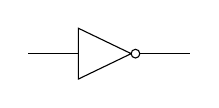
\begin{tikzpicture}[circuit logic US, scale=0.9]
\node[not gate, draw] (n) {};
\draw (n.input) -- ++(-0.7,0);
\draw (n.output) -- ++(0.7,0);
\end{tikzpicture}

\[
Y=\overline{A}
\]

\begin{tabular}{c|c}
\toprule
A & Y\\
\midrule
0 & 1\\
1 & 0\\
\bottomrule
\end{tabular}
\end{minipage}
\hfill
\begin{minipage}[t]{0.32\textwidth}
\centering
\textbf{AND}

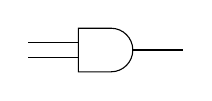
\begin{tikzpicture}[circuit logic US, scale=0.9]
\node[and gate, draw] (n) {};
\draw (n.input 1) -- ++(-0.7,0);
\draw (n.input 2) -- ++(-0.7,0);
\draw (n.output) -- ++(0.7,0);
\end{tikzpicture}

\[
Y=AB
\]

\begin{tabular}{cc|c}
\toprule
A & B & Y\\
\midrule
0 & 0 & 0\\
0 & 1 & 0\\
1 & 0 & 0\\
1 & 1 & 1\\
\bottomrule
\end{tabular}
\end{minipage}
\hfill
\begin{minipage}[t]{0.32\textwidth}
\centering
\textbf{OR}

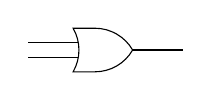
\begin{tikzpicture}[circuit logic US, scale=0.9]
\node[or gate, draw] (n) {};
\draw (n.input 1) -- ++(-0.7,0);
\draw (n.input 2) -- ++(-0.7,0);
\draw (n.output) -- ++(0.7,0);
\end{tikzpicture}

\[
Y=A+B
\]

\begin{tabular}{cc|c}
\toprule
A & B & Y\\
\midrule
0 & 0 & 0\\
0 & 1 & 1\\
1 & 0 & 1\\
1 & 1 & 1\\
\bottomrule
\end{tabular}
\end{minipage}
\end{center}

\begin{center}
\begin{minipage}[t]{0.32\textwidth}
\centering
\textbf{XOR}

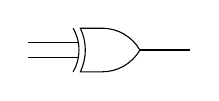
\begin{tikzpicture}[circuit logic US, scale=0.9]
\node[xor gate, draw] (n) {};
\draw (n.input 1) -- ++(-0.7,0);
\draw (n.input 2) -- ++(-0.7,0);
\draw (n.output) -- ++(0.7,0);
\end{tikzpicture}

\[
Y=A\oplus B
\]

\begin{tabular}{cc|c}
\toprule
A & B & Y\\
\midrule
0 & 0 & 0\\
0 & 1 & 1\\
1 & 0 & 1\\
1 & 1 & 0\\
\bottomrule
\end{tabular}
\end{minipage}
\hfill
\begin{minipage}[t]{0.32\textwidth}
\centering
\textbf{NAND}

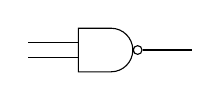
\begin{tikzpicture}[circuit logic US, scale=0.9]
\node[nand gate, draw] (n) {};
\draw (n.input 1) -- ++(-0.7,0);
\draw (n.input 2) -- ++(-0.7,0);
\draw (n.output) -- ++(0.7,0);
\end{tikzpicture}

\[
Y=\overline{AB}
\]

\begin{tabular}{cc|c}
\toprule
A & B & Y\\
\midrule
0 & 0 & 1\\
0 & 1 & 1\\
1 & 0 & 1\\
1 & 1 & 0\\
\bottomrule
\end{tabular}
\end{minipage}
\hfill
\begin{minipage}[t]{0.32\textwidth}
\centering
\textbf{NOR}

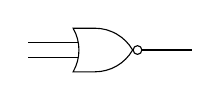
\begin{tikzpicture}[circuit logic US, scale=0.9]
\node[nor gate, draw] (n) {};
\draw (n.input 1) -- ++(-0.7,0);
\draw (n.input 2) -- ++(-0.7,0);
\draw (n.output) -- ++(0.7,0);
\end{tikzpicture}

\[
Y=\overline{A+B}
\]

\begin{tabular}{cc|c}
\toprule
A & B & Y\\
\midrule
0 & 0 & 1\\
0 & 1 & 0\\
1 & 0 & 0\\
1 & 1 & 0\\
\bottomrule
\end{tabular}
\end{minipage}
\end{center}

% ---------------------------------
\subsection{NANDゲート}
% ---------------------------------

NAND ゲートは AND ゲートの出力を否定したものである。


\[
Y = \overline{AB}
\]

NAND ゲートは \textbf{万能ゲート}であり、
NAND のみを用いてすべての論理回路を構成できる。

ド・モルガンの法則より、

\[
\overline{AB} = \overline{A} + \overline{B}
\]

と書き換えることができる。

% ---------------------------------
\subsection{NORゲート}
% ---------------------------------

NOR ゲートは OR ゲートの出力を否定したものである。

\[
Y = \overline{A + B}
\]

こちらも NAND と同様に万能ゲートである。

ド・モルガンの法則を用いると、

\[
\overline{A + B} = \overline{A}\,\overline{B}
\]

と表せる。

% ---------------------------------
\subsection{XORゲート}
% ---------------------------------

XOR は「入力が異なるときに 1 となる」論理である。

\[
Y = A \oplus B
\]

AND / OR / NOT を用いて展開すると、

\[
Y = \overline{A}B + A\overline{B}
\]

となる。



\section{真理値表とカルノー図}
% ---------------------------------
\subsection{真理値表から論理式を作る}
% ---------------------------------

真理値表から論理式を作る手順を以下の真理値表を例にとって考える。
手順は以下に示す。

\begin{enumerate}
  \item 出力が 1 となる入力の組を探す
  \item それぞれを AND 項として書き出す
  \item OR でまとめる
\end{enumerate}

\begin{center}
\begin{tabular}{ccc|c}
\toprule
A & B & C & Y \\
\midrule
0 & 0 & 0 & 0 \\
1 & 0 & 0 & 0 \\
0 & 1 & 0 & 0 \\
0 & 0 & 1 & 0 \\
1 & 1 & 0 & 1 \\
1 & 0 & 1 & 1 \\
0 & 1 & 1 & 1 \\
1 & 1 & 1 & 1 \\
\bottomrule
\end{tabular}
\end{center}

この真理値表から、
\[
\begin{aligned}
Y &= AB\overline{C} + A\overline{B}C + \overline{A}BC + ABC \\
  &= AB\overline{C} + A\overline{B}C + \overline{A}BC + (ABC + ABC + ABC) \\
  &= (AB\overline{C} + ABC) + (A\overline{B}C + ABC) + (\overline{A}BC + ABC) \\
  &= AB(\overline{C} + C) + AC(\overline{B} + B) + BC(\overline{A} + A) \\
  &= AB + AC + BC
\end{aligned}
\]
が得られる。これは、3入力多数決回路と呼ばれるものである。論理ゲートの図で表現したものを以下に示す。\\
3入力多数決回路（Majority Circuit）は，
3つの入力 $A,B,C$ のうち
\textbf{2つ以上が 1 のときに 1 を出力する}回路である。この回路は AND と OR のみで構成できる。このように、論理式を直接変形することで簡単にすることもできるが、カルノー図を使って直観的に簡単な形ににもっていくこともできる。

% ---------------------------------
\subsection{カルノー図の作成}
% ---------------------------------
カルノー図とは論理式を簡略化するために用いられる記法である。
まず，入力変数 $A,B$ を横軸，
$C$ を縦軸とする 3 変数カルノー図を作成する。
横軸はグレイコード順（00,01,11,10）で配置する。

\begin{center}
\begin{tabular}{c|cccc}
$C \backslash AB$ & 00 & 01 & 11 & 10 \\
\hline
0 & 0 & 0 & 1 & 0 \\
1 & 0 & 1 & 1 & 1 \\
\end{tabular}
\end{center}

% ---------------------------------
\subsection{グルーピング}
% ---------------------------------

カルノー図上で 1 が配置されているセルを，
2のべき乗個（1,2,4,8,...）でまとめる。

\begin{itemize}
  \item $AB=11$ の列は $C=0,1$ で 1 → $AB$
  \item $AC=11$ に対応する 2 セル → $AC$
  \item $BC=11$ に対応する 2 セル → $BC$
\end{itemize}

これにより，最小論理式が得られる。

% ---------------------------------
\subsection{最小論理式}
% ---------------------------------

\[
Y = AB + AC + BC
\]

最小論理式とは最も簡単にかける論理式のことである。この式は，「3つのうち 2つが 1」という3入力多数決の条件をそのまま表していることが分かる。

% =================================
\section{2進数の表現}
% =================================
10進数の数の場合、一桁目は10の0乗の位、二桁目は10の1乗の位、三桁目は10の2乗の位・・・と対応して考えることができる。同様に2進数の数の場合、一桁目は2の0乗の位、二桁目は2の1乗の位、三桁目は2の2乗の位・・・と対応して考えることができる。\\
例)\quad$(2)_{10} \,→\, (10)_2$\quad\,\,$(11)_{10}\,→\, (1011)_2$\quad\,\,$(35)_{10}\,→\, (100011)_2$
% =================================
\section{2進数の加算の基本}
% =================================
ここでは、2進数の加算を筆算で行い、
それがどのように論理演算（ブール演算）で
実現されているかを説明する。10進数の時と同様、桁毎に演算を行うが、繰り上がりに注意する必要がある。
10進数では 9+1 で繰り上がりが発生するが、
2進数では 1+1 で繰り上がりが発生する。


\[
\begin{array}{cccc}
 & 1 & 0 & 1 \\
+& 0 & 1 & 1 \\
\hline
1 & 0 & 0 & 0
\end{array}
\]

この計算は、下位ビットから順に処理されている。

% ---------------------------------
\subsection{1ビット加算の考え方}
% ---------------------------------

1ビット同士の加算を考える。
入力を $A,B$ とすると、次の 2 つの出力が必要になる。

\begin{itemize}
  \item 和（Sum）
  \item 桁上がり（Carry）
\end{itemize}

\begin{center}
\begin{tabular}{cc|cc}
\toprule
A & B & Sum & Carry \\
\midrule
0 & 0 & 0 & 0 \\
0 & 1 & 1 & 0 \\
1 & 0 & 1 & 0 \\
1 & 1 & 0 & 1 \\
\bottomrule
\end{tabular}
\end{center}

この表は、前章で説明した半加算器の真理値表と一致する。

% ---------------------------------
\subsection{ブール演算として見る加算}
% ---------------------------------

上の真理値表から、それぞれの出力は次の論理式で表される。

\begin{align*}
\text{Sum} &= A \oplus B \\
\text{Carry} &= AB
\end{align*}

すなわち、2進数の加算は
\textbf{XOR と AND の組み合わせ}として実現される。

% ---------------------------------
\subsection{桁上がりを含む加算}
% ---------------------------------

次に、桁上がりを含む 1 ビット加算を考える。
入力は $A,B$ に加えて、下位桁からの桁上がり $C_{\text{in}}$ がある。

\[
\begin{array}{cccc}
 & 1 & 0 & 1 \\
+& 0 & 1 & 1 \\
\hline
1 & 0 & 0 & 0
\end{array}
\]

右端の計算では

\[
1 + 1 = 0 \quad (\text{Carry } 1)
\]

となり、この Carry が次の桁へ渡される。

\subsection{半加算器（HA）}

半加算器は、2つの 1 ビット入力 $A,B$ を加算し，
和（Sum）と桁上がり（Carry）を出力する回路である。

\subsection*{論理演算の考え方}

\begin{itemize}
  \item 和（Sum）は，$A$ と $B$ が異なるときに 1
  \item 桁上がり（Carry）は，$A$ と $B$ が両方 1 のときに 1
\end{itemize}

よって，論理式は次のようになる。

\begin{align*}
\text{Sum} &= A \oplus B \\
\text{Carry} &= AB
\end{align*}

\subsection*{論理ゲート図}
\begin{center}
\usetikzlibrary{circuits.logic.US}
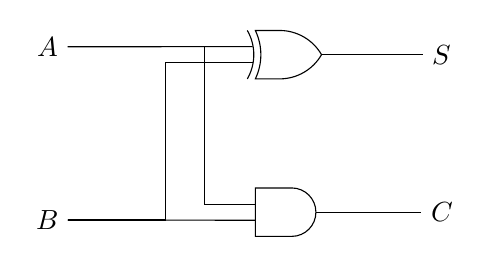
\begin{tikzpicture}[circuit logic US]

% Inputs
\node (A) at (0,0.1) {$A$};
\node (B) at (0,-2.1) {$B$};

% XOR gate (Sum)
\node[xor gate, draw, logic gate inputs=nn] 
  (XOR) at (3,0) {};

% AND gate (Carry)
\node[and gate, draw, logic gate inputs=nn] 
  (AND) at (3,-2) {};

% Outputs
\node (S) at (5,0) {$S$};
\node (C) at (5,-2) {$C$};

% Connections
\draw (A) -- (XOR.input 1);
\draw (B) -- (AND.input 2);
\draw (B) -- ++(1.5,0) |- (XOR.input 2);
\draw (A) -- ++(2,0) |- (AND.input 1);

\draw (XOR.output) -- (S);
\draw (AND.output) -- (C);

\end{tikzpicture}
\end{center}



\subsection*{真理値表}

\begin{center}
\begin{tabular}{cc|cc}
\toprule
A & B & Sum & Carry \\
\midrule
0 & 0 & 0 & 0 \\
0 & 1 & 1 & 0 \\
1 & 0 & 1 & 0 \\
1 & 1 & 0 & 1 \\
\bottomrule
\end{tabular}
\end{center}

\subsection{全加算器（FA）}

全加算器は，入力 $A,B$ に加えて，
下位桁からの桁上がり $C_{\text{in}}$ を含めて加算を行う回路である。

\subsection*{論理演算の考え方}

\begin{itemize}
  \item 和（Sum）は，3入力のうち 1 の個数が奇数のときに 1
  \item 桁上がり（Carry）は，2つ以上が 1 のときに 1
\end{itemize}

これより，論理式は次のように表される。

\begin{align*}
\text{Sum} &= A \oplus B \oplus C_{\text{in}} \\
\text{Carry} &= AB + C_{\text{in}}(A \oplus B)
\end{align*}

\subsection*{論理ゲート図}

\begin{center}
  \begin{tikzpicture}[circuit logic US]
    % Half adder 2
    \draw (4,1) node[xor gate] (xor2) {};
    \draw (xor2)+(0,1) node[and gate] (and2) {};

    % Half adder 1
    \draw (and2.input 1)+(-2,0) node[xor gate] (xor1) {};
    \draw (xor1)+(0,1) node[and gate] (and1) {};

    % Carry
    \draw ($0.5*(and1)+0.5*(and2)+(3,0)$) node[or gate] (or) {};

    % connection between AND1 and XOR1
    \draw (and1.input 1) to ++(-0.70,0) node [branch] {} |- (xor1.input 1);
    \draw (and1.input 2) to ++(-0.35,0) node [branch] {} |- (xor1.input 2);

    % connection between HA1 and HA2
    \draw (xor1.output) -- (and2.input 1);

    % connection between AND1 and XOR1
    \draw (xor1.output)  to ++( 0.70,0) node [branch] {} |- (xor2.input 1);
    \draw (xor2.input 2) to ++(-0.35,0) node [branch] {} |- (and2.input 2);

    % connection between AND1,2 and OR
    \draw (or.input 2) -- ++(-0.4,0) |- (and2.output);
    \draw (or.input 1) -- ++(-0.4,0) |- (and1.output);

    % outputs
     \draw (or.output) -- ++(1,0) node[right] (output) {$Carry$};
     \draw (xor2.output) -- ($($(or.output)+(1,0)$)!(xor2.output)!($(or.output)+(1,1)$)$) node[right] {$Sum$};

    % inputs
     \draw (xor2.input 2) -- ($(0,1)!(xor2.input 2)!(0,0)$) node[left] {$C_{in}$};
     \draw (and1.input 1) -- ($(0,1)!(and1.input 1)!(0,0)$) node[above] {$A$};
     \draw (and1.input 2) -- ($(0,1)!(and1.input 2)!(0,0)$) node[below] {$B$};
  \end{tikzpicture}
\end{center}

\subsection*{真理値表}

\begin{center}
\begin{tabular}{ccc|cc}
\toprule
A & B & $C_{\text{in}}$ & Sum & Carry \\
\midrule
0 & 0 & 0 & 0 & 0 \\
0 & 0 & 1 & 1 & 0 \\
0 & 1 & 0 & 1 & 0 \\
0 & 1 & 1 & 0 & 1 \\
1 & 0 & 0 & 1 & 0 \\
1 & 0 & 1 & 0 & 1 \\
1 & 1 & 0 & 0 & 1 \\
1 & 1 & 1 & 1 & 1 \\
\bottomrule
\end{tabular}
\end{center}

% =================================
\section{おまけ}
% =================================

本章では，加算器を基にした減算の方法と，
複数ビット加算における時間的な問題について解説する。

% ---------------------------------
\subsection{減算器の考え方}
% ---------------------------------

2進数の減算 $A - B$ は，
2の補数表現を用いることで加算として処理できる。

\[
A - B = A + (\overline{B} + 1)
\]

ここで，$\overline{B}$ は $B$ の各ビットを反転したものである。

この式から分かるように，
減算器は「反転器（NOT）」と「加算器」の組み合わせとして構成できる。

\subsection*{減算回路の構成}

\begin{itemize}
  \item $B$ の各ビットを NOT ゲートで反転する
  \item 初段のキャリー入力に 1 を与える
  \item あとは通常の加算器として処理する
\end{itemize}

この構成により，加算器と減算器を
同一の回路で兼用することが可能になる。

% ---------------------------------
\subsection{リップルキャリー加算器}
% ---------------------------------

複数ビットの加算は，
全加算器を桁ごとに直列接続することで実現される。
この構成を \textbf{リップルキャリー加算器} と呼ぶ。

\begin{figure}[h]
\centering
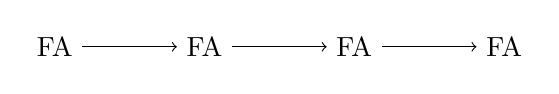
\begin{tikzpicture}
\node (fa1) {FA};
\node[right=1.2cm of fa1] (fa2) {FA};
\node[right=1.2cm of fa2] (fa3) {FA};
\node[right=1.2cm of fa3] (fa4) {FA};
\draw[->] (fa1) -- (fa2);
\draw[->] (fa2) -- (fa3);
\draw[->] (fa3) -- (fa4);
\end{tikzpicture}
\caption{リップルキャリー加算器の概念図}
\end{figure}

各桁のキャリー出力が次の桁へ順番に伝播するため，
キャリーは波（ripple）のように流れていく。

% ---------------------------------
\subsection{処理時間の問題}
% ---------------------------------

リップルキャリー加算器の最大の欠点は，
計算に時間がかかる点である。

最下位ビットで発生したキャリーは，
すべての桁を通過しなければ
最上位ビットの結果が確定しない。

そのため，ビット数が増えるほど，
遅延時間は次のように増加する。

\[
\text{遅延時間} \propto \text{ビット数}
\]

これは，高速な演算が求められる回路では
大きな問題となる。

% ---------------------------------
\subsection{高速化へのアプローチ}
% ---------------------------------

この問題を解決するために，
以下のような手法が考えられている。

\begin{itemize}
  \item キャリー先読み加算器（Carry Lookahead Adder）
  \item 桁ごとにキャリーを予測する構成
  \item 並列処理による遅延の削減
\end{itemize}

詳細な回路構成は複雑になるため本書では省略するが，
「速さ」と「回路規模」のトレードオフが存在することは
重要なポイントである。%論理回路とは何か
%基礎電気回路理論
\chapter{基礎電気回路理論}


本書では、電磁気学の基礎法則から出発し、
電気回路としてそれらがどのように表現されるかを学んできた。
本章では、回路理論の要点を整理し、各概念の関係をまとめる。

\section{電圧・電流・回路素子}

回路理論では、主に電圧 $V$、電流 $I$、電荷 $Q$ を基本量として扱う。

\begin{itemize}
\item 電流は電荷の時間変化として定義される
\begin{equation}
I = \frac{dQ}{dt}
\end{equation}

\item 電圧はエネルギーの差を表す量であり、
電場の線積分として定義される
\begin{equation}
V = -\int \vec{E} \cdot d\vec{l}
\end{equation}
\end{itemize}

これらの量を結びつける要素として、
抵抗、コンデンサ、コイルが導入される。



\section{基本回路素子}

\subsection{抵抗}

抵抗は電流と電圧を比例関係で結ぶ素子であり、
オームの法則に従う。

\begin{equation}
V = RI
\end{equation}

抵抗はエネルギーを熱として消費する散逸素子である。



\subsection{コンデンサ}

コンデンサは電荷を蓄える素子であり、
電圧と電荷の関係は

\begin{equation}
Q = CV
\end{equation}

で表される。
エネルギーは電場として蓄えられる。



\subsection{コイル}

コイルは電流の変化に対して起電力を生じる素子であり、

\begin{equation}
V = L\frac{dI}{dt}
\end{equation}

で表される。
エネルギーは磁場として蓄えられる。



\section{キルヒホッフの法則}

回路全体の振る舞いは、以下の二つの法則によって記述される。

\begin{itemize}
\item 電流則（KCL）：節点における電流の保存
\begin{equation}
\sum I = 0
\end{equation}

\item 電圧則（KVL）：閉回路におけるエネルギー保存
\begin{equation}
\sum V = 0
\end{equation}
\end{itemize}

これらは、それぞれ電荷保存則とエネルギー保存則に基づいている。



\section{時間応答と過渡現象}

RC回路やRL回路では、
回路量は時間に依存して変化し、指数関数的な応答を示す。

\begin{equation}
e^{-t/\tau}
\end{equation}

で表される時定数 $\tau$ は、
回路の応答速度を決定する重要な指標である。



\section{交流回路とインピーダンス}

交流回路では、電圧と電流は時間的に変動するため、
複素数表示を用いた解析が有効である。

各素子のインピーダンスは

\begin{align}
Z_R &= R \\
Z_L &= j\omega L \\
Z_C &= \frac{1}{j\omega C}
\end{align}

で定義され、
直列回路では単純に加算される。



\section{電磁気学とのつながり}

回路理論は電磁気学の近似として理解できる。

\begin{itemize}
\item 電圧：電場の線積分
\item 電流：電荷の流れ
\item インダクタンス：電磁誘導
\item コンデンサ：電場エネルギー
\end{itemize}

特にキルヒホッフの法則は、
マクスウェル方程式を回路スケールで近似した結果とみなせる。

\section{その他重要な知識}
\subsection{抵抗分圧}

直列に接続された抵抗に電圧を加えると、
各抵抗にかかる電圧は抵抗値に比例して分配される。
これを抵抗分圧という。


\begin{figure}[h]
    \centering
    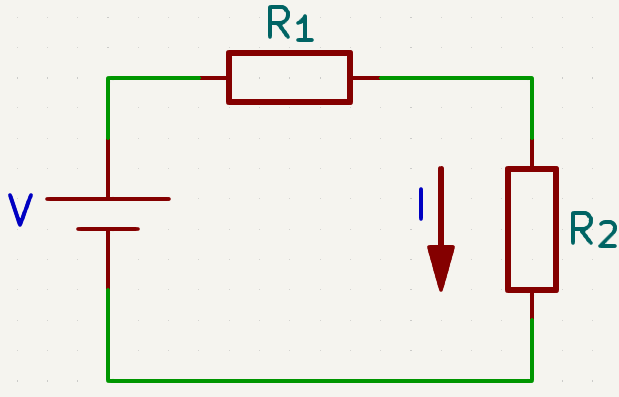
\includegraphics[width=0.5\textwidth]{circuit_theory/voltage_divider.png}
    \caption{抵抗分圧回路の例}
    \label{fig:voltage_divider}
\end{figure}

\subsection{分圧の式}

直列回路では電流は共通であり、

\begin{equation}
I = \frac{V_{\mathrm{in}}}{R_1 + R_2}
\end{equation}

である。

抵抗 $R_2$ にかかる電圧（出力電圧）は

\begin{align}
V_{\mathrm{out}}
&= I R_2 \\
&= \frac{R_2}{R_1 + R_2} V_{\mathrm{in}}
\end{align}

となる。

特に、$R_1 = 0$ の場合、$V_{\mathrm{out}} = V_{\mathrm{in}}$ となり、
$R_2 = 0$ の場合、$V_{\mathrm{out}} = 0$ となる。

また、$R_1 = \infty$ の場合、$V_{\mathrm{out}} = 0$ となり、
$R_2 = \infty$ の場合、$V_{\mathrm{out}} = V_{\mathrm{in}}$ となる。


\subsection{二端子対回路}
ある線形な回路網に対して、その回路網の両端に接続された二つの端子対に注目することができる。(図\ref{fig:two_port_network}参照)

\begin{figure}[htbp]
    \centering
    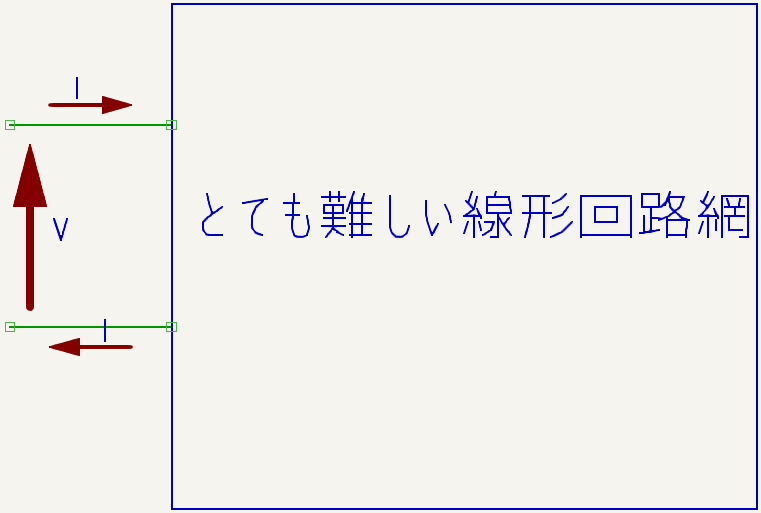
\includegraphics[width=0.5\textwidth]{circuit_theory/two_port_network.png}
    \caption{二端子対回路の概念図}
    \label{fig:two_port_network}
\end{figure}

このような二端子対に対して、電圧$V$と電流$I$の関係にのみ着目すれば、内部の複雑な回路構成を無視して、二端子対を一つの素子として扱うことができる。
\newpage
\subsection{入出力インピーダンス}

二端子対回路の考え方を応用したものとして、入力インピーダンスと出力インピーダンスの概念がある。

ある回路網の二端子対に交流信号を印加したとき、その二端子対に流れる電流($I$)と電圧($V$)に対して、入力インピーダンスとは、
\begin{align}
    Z_{in} = \frac{V}{I}
\end{align}
で定義される。
このとき、二端子対回路は、交流信号源から見たときに、抵抗値$Z_{in}$を持つ素子として振る舞うことになる。(図\ref{fig:input_impedance}参照)
\begin{figure}[htbp]
    \centering
    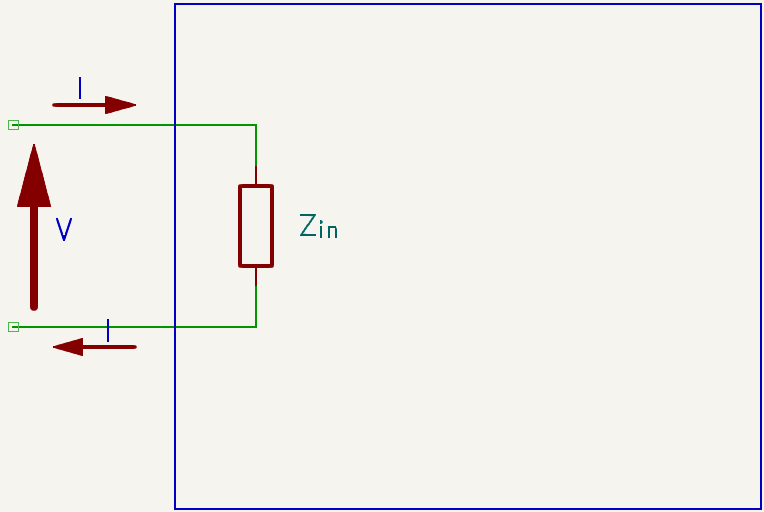
\includegraphics[width=0.5\textwidth]{circuit_theory/input_impedance.png}
    \caption{入力インピーダンスの概念図}
    \label{fig:input_impedance}
\end{figure}

同様に、ある回路網が電源として、二端子に電力を供給しているとき、起電力$E$と出力インピーダンス$Z_{out}$は、図\ref{fig:output_impedance}のように表される。
\begin{figure}[htbp]
    \centering
    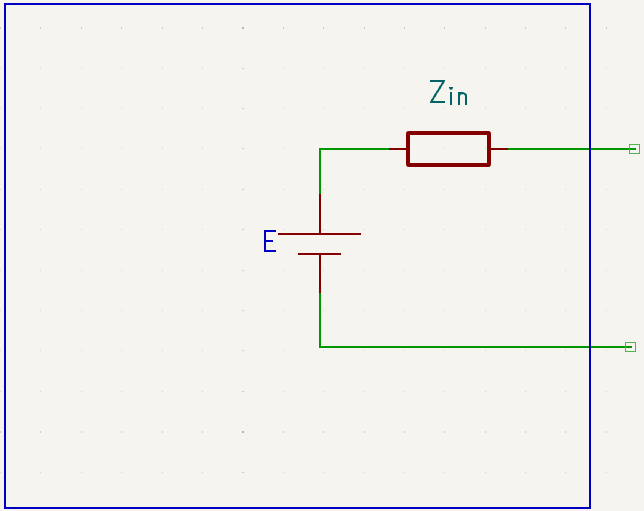
\includegraphics[width=0.5\textwidth]{circuit_theory/output_impedance.png}
    \caption{出力インピーダンスの概念図}
    \label{fig:output_impedance}
\end{figure}

入力インピーダンスは素子の入力側から見た特性を表し、高いほど電流を消費しないため良いとされている。
一方、出力インピーダンスは素子の出力側から見た特性を表し、低いほど負荷に対して安定した電圧を供給できるため良いとされている。
%基礎回路理論
%トランジスタ等素子の説明
\chapter{各種素子の動作原理}
\section{半導体}
半導体とは、絶縁体に違う種類の不純物をドープすることによって導電性を持たせた材料である。代表的な半導体材料としてシリコン(Si)やゲルマニウム(Ge)がある。
半導体はドープする不純物の種類によって、p型半導体とn型半導体に分類される。
最外殻電子が4個のシリコンに、最外殻電子が5個のリン(P)などの不純物をドープすると、余分な電子が導電に寄与するためn型半導体となる。
一方、最外殻電子が3個のホウ素(B)などの不純物をドープすると、電子が不足するため正孔が導電に寄与し、p型半導体となる。



\section{ダイオードの動作原理}
ダイオードは図\ref{fig:diode_section}のようにp型半導体とn型半導体を接合して作られた素子である。
\begin{figure}[htbp]
    \centering
    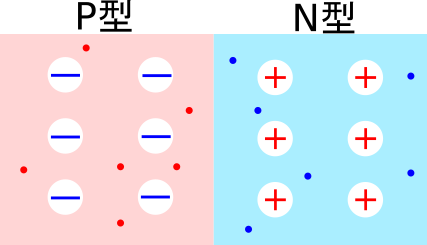
\includegraphics[width=0.5\textwidth]{graphit/diode.png}
    \caption{ダイオードの断面図}
    \label{fig:diode_section}
\end{figure}
ここで、図\ref{fig:diode_section}のP型のほうにある小さい丸は正孔を、N型のほうにある小さい丸は電子を表している。
また、P型のほうにある大きい丸は正孔が移動することによってできた負の固定電荷を、N型のほうにある大きい丸は自由電子が移動することによってできた正の固定電荷を表している。

これらの自由電子と正孔は自由に動くことができるため勝手に拡散し、P型半導体とN型半導体との境界付近で、自由電子と正孔が再結合する。(図\ref{fig:diode_diffusion}参照)
\begin{figure}[htbp]
    \begin{minipage}
        {0.45\hsize}
        \centering
        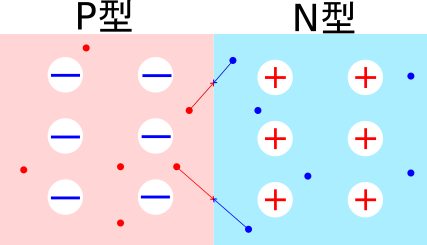
\includegraphics[width=0.8\textwidth]{graphit/diode_extinction.png}
        \caption{ダイオードにおける自由電子と正孔の再結合}
        \label{fig:diode_diffusion}
    \end{minipage}
    \begin{minipage}
        {0.45\hsize}
        \centering
        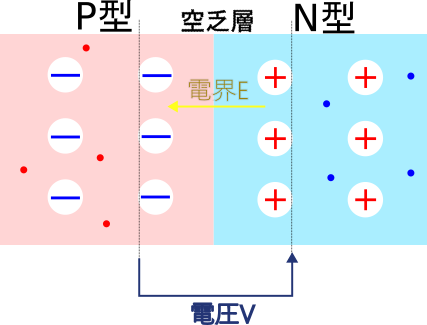
\includegraphics[width=0.8\textwidth]{graphit/diode_depletion.png}
        \caption{ダイオードにおける空乏層の形成}
        \label{fig:diode_depletion}
    \end{minipage}
\end{figure}

この再結合が進むと、境界付近には自由電子と正孔がいなくなり、固定電荷だけが残る領域ができる。この領域を空乏層と呼ぶ。(図\ref{fig:diode_depletion}参照)

この領域には固定電荷が残っていいるため、これによる電界がN型半導体側からP型半導体側に向かって発生する。この電界は自由電子と正孔の拡散を妨げる向きに働くため、自由電子と正孔の拡散が止まり、
空乏層の拡大も止まる。ここの電位差を拡散電位(built-in potential)と呼び、P型半導体とN型半導体とのフェルミ準位の差に等しい。

ここで、電圧をN側を正として印加することを考えてみると、空乏層と同じ方向の電界が発生するため、空乏層を大きくする方法に働き、電流は少ししか流れない。
ここで電流が少ししか流れないといったが、実は、P型半導体にはメインキャリアの正孔の他に少数キャリアの電子が存在し、N型半導体には少数キャリアの正孔が存在する。
これらは熱励起などによって生成されるため、少数キャリアは常に存在する。この少数キャリアが空乏層を通過することによって、逆方向にもわずかな電流が流れる。

次に、電圧をP側を正として印加してみると、空乏層と逆方向の電界が発生するため、空乏層を小さくする方向に働き、自由電子と正孔が空乏層を通過しやすくなる。
その結果、大きな電流が流れるようになる。このように、ダイオードは一方向にのみ大きな電流を流す素子である。
なお、P型半導体側をアノード、N型半導体側をカソードと呼ぶ。

ダイオードの電圧-電流特性は
\begin{align}
    I_D = I_S \left\{ \exp{\left(\frac{eV}{k_bT}\right)} - 1 \right\}
\end{align}
という風に表される。(図\ref{fig:diode_specific})ここで、$I_D$はダイオード電流、$I_S$は逆方向飽和電流、$e$は素電荷、$V$はダイオードにかかる電圧、$k_b$はボルツマン定数、$T$は絶対温度である。
室温付近では大体$V_T = k_bT/e \approx 26mV$である。
\begin{figure}[htbp]
    \centering
    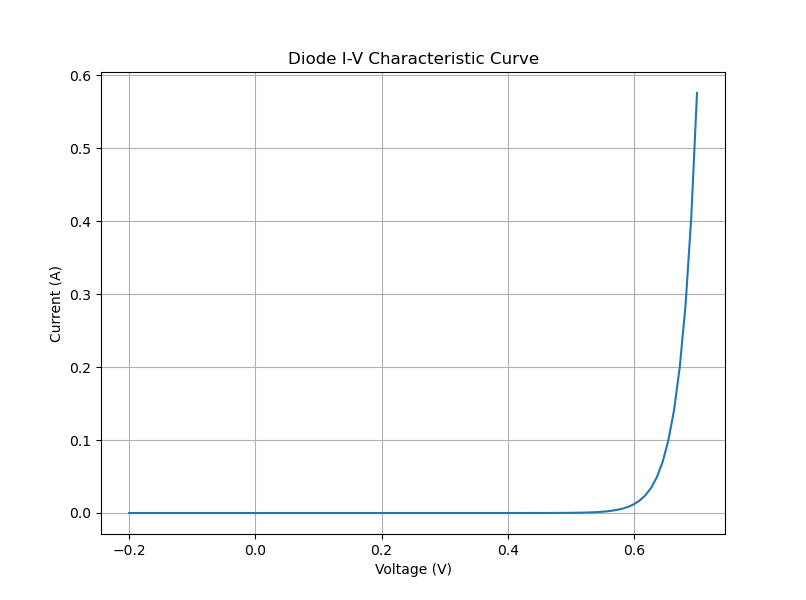
\includegraphics[width=0.8\textwidth]{diode_IV.png}
    \caption{ダイオードの電圧-電流特性($I_S = 10^{-12}$A,$V_T = 25.85$mV)}
    \label{fig:diode_specific}
\end{figure}
\newpage

図\ref{fig:diode_specific}からわかるように、ダイオードは順方向に約0.7V以上の電圧がかかると急激に電流が流れ始める特性を持っている。

% \subsection{ダイオードのコラム}
% ツェナー降伏とかアノード・カソードとか真空管とか


\section{バイポーラトランジスタの動作原理}
バイポーラトランジスタ(以下BJT)は、3つの半導体領域を接合して作られた素子である。NPN型とPNP型の2種類があるが、ここではNPN型について説明する。 図\ref{fig:bjt_section}にBJTの断面図を示す。
\begin{figure}[htbp]
    \centering
    \includegraphics[width=0.5\textwidth]{graphit/bjt.png}
    \caption{バイポーラトランジスタの断面図}
    \label{fig:bjt_section}
\end{figure}
BJTはエミッタ(E)、ベース(B)、コレクタ(C)の3つの端子を持つ。エミッタはn型半導体、ベースはp型半導体、コレクタはn型半導体で構成されているが、コレクタのn型半導体のドープ濃度はエミッタのn型半導体のドープ濃度よりも低い。

N型半導体とP型半導体の接合部にはダイオードと同じようにそれぞれ空乏層が形成される。

ここでエミッタからベースに電圧を印加し、ベース電流$I_B$を流すと、エミッタベース間のエミッタベース間の空乏層がつぶれ、エミッタからベースに向かって多数キャリアである電子が注入される。
ベースはp型半導体であるため、注入された電子は正孔と再結合するが、
ここでベースコレクタ間に電圧を印加すると、ベースが十分に薄い場合、エミッタからベースに向かっていた電子のほとんどはコレクタベース間の空乏層に存在する電界の影響を受けてコレクタに引き寄せられ、
コレクタ電流$I_C$として流れる。(図\ref{fig:bjt_operation}参照)
\begin{figure}[htbp]
    \centering
    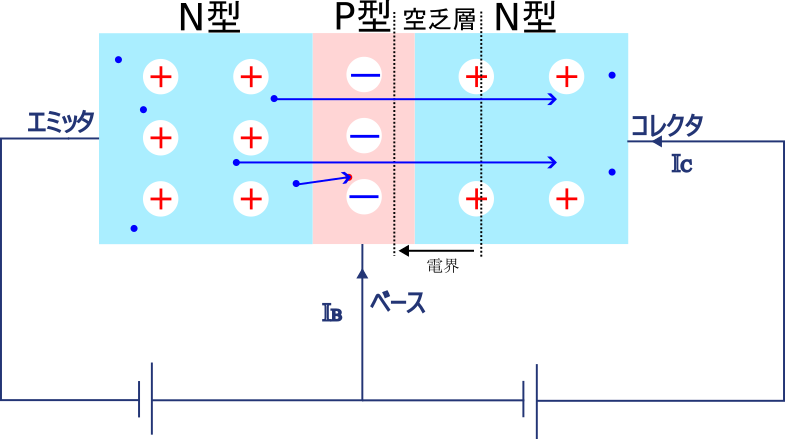
\includegraphics[width=0.5\textwidth]{graphit/bjt_operation.png}
    \caption{バイポーラトランジスタの動作原理}
    \label{fig:bjt_operation}
\end{figure}
このとき、エミッタ電流$I_E$はキルヒホッフの法則より、
\begin{align}
    I_E = I_B + I_C
\end{align}
である。また、エミッタから出発してコレクタに到達する電子の割合を$\alpha$とすると、
\begin{align}
    I_C = \alpha I_E
\end{align}
である。よって
\begin{align}
    I_C = \frac{\alpha}{1 - \alpha} I_B
\end{align}
となる。ここで、$\beta = \frac{\alpha}{1 - \alpha}$をBJTの電流増幅率と呼ぶ。
$\alpha$は0以上1未満の値をとるため、$\beta$は1以上の値をとる。通常、$\beta$は100程度の値をとるため、小さいベース電流$I_B$で大きなコレクタ電流$I_C$を制御することができる。

また、PNP型のBJTはNPN型BJTと同様の動作原理で動作する。

余談ではあるが、トランジスタのベースエミッタ間はN型半導体とP型半導体の接合部であるため、ダイオードと同様の電圧-電流特性を持つ。

\section{MOSFETの動作原理}
MOSFETは、金属酸化被膜電界効果トランジスタ(Metal-Oxide-Semiconductor Field Effect Transistor)の略であり、電界効果を利用して動作するトランジスタである。
MOSFETにはnチャネル型とpチャネル型の2種類があるが、ここではnチャネル型について説明する。図\ref{fig:mosfet_section}にMOSFETの断面図を示す。
\begin{figure}[htbp]
    \centering
    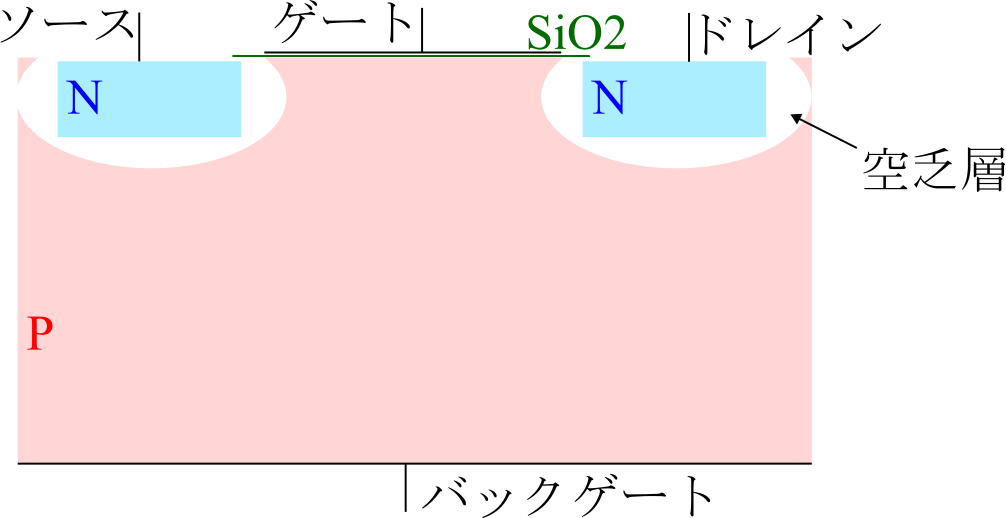
\includegraphics[width=0.5\textwidth]{graphit/mosfet.png}
    \caption{MOSFETの断面図}
    \label{fig:mosfet_section}
\end{figure}
MOSFETはソース(S)、ドレイン(D)、ゲート(G)、およびバックゲート(BG)の4つの端子を持つ。ソースとドレインはn型半導体で構成されている。
また、ゲートは絶縁膜(通常はSiO2)を介して基板に接続された金属電極である。
また、多くのMOSFETではバックゲート端子はソース端子に接続されている。
ここでゲートソース間に正の電圧$V_{GS}$を印加すると、基板内のp型半導体領域に電界が発生し、
p型半導体内部の少数キャリアである電子がゲート下に引き寄せられ、まるでn型としてふるまう反転層が形成される。
この反転層はソースとドレインを接続する導電チャネルとなるため、ドレインソース間に電圧$V_{DS}$を印加すると、ドレインからソースに向かって電子が流れ、ドレイン電流$I_D$が流れる。(図\ref{fig:mosfet_operation}参照)
\begin{figure}[htbp]
    \centering
    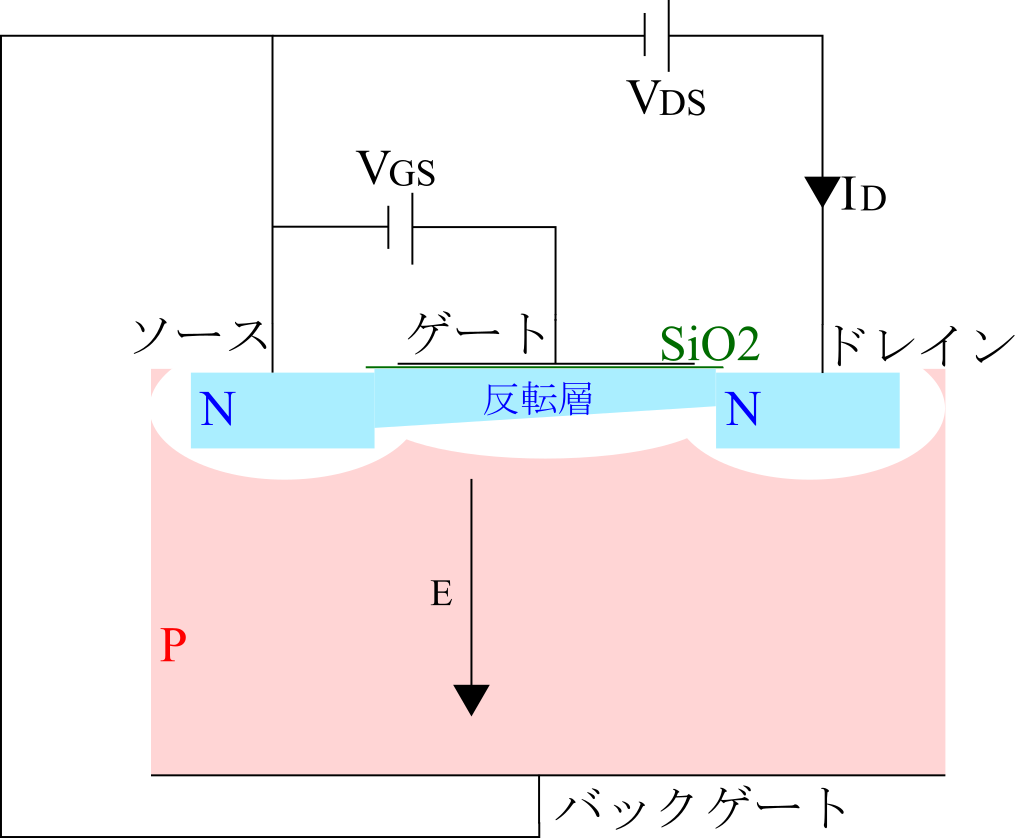
\includegraphics[width=0.5\textwidth]{graphit/mosfet_operation.png}
    \caption{MOSFETの動作原理}
    \label{fig:mosfet_operation}
\end{figure}
動作原理より、BJTと違って電流ではなくゲートソース間電圧$V_{GS}$によってドレイン電流$I_D$を制御することができる。

余談ではあるが、MOSFETのバックゲート=ソースとドレイン間にはpn接合が形成されているため、ダイオードと同様の電圧-電流特性を持つ。
この、バックゲート=ソースとドレイン間のpn接合を寄生ダイオード(ボディダイオード)と呼ぶ。


% \section{メカニカルリレーの動作原理}

\section{それぞれの回路での扱い方}
図\ref{fig:diode_cir},\ref{fig:bjt_cir},\ref{fig:mosfet_cir}にダイオード、BJT、MOSFETの回路記号を示す。
\begin{figure}[htbp]
    \begin{minipage}
        {0.3\hsize}
        \centering
        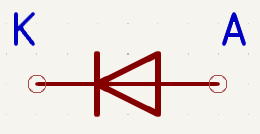
\includegraphics[width=0.5\textwidth]{graphit/diode_circuit.png}
        \caption{ダイオードの回路記号}
        \label{fig:diode_cir}
    \end{minipage}
    \begin{minipage}
        {0.3\hsize}
        \centering
        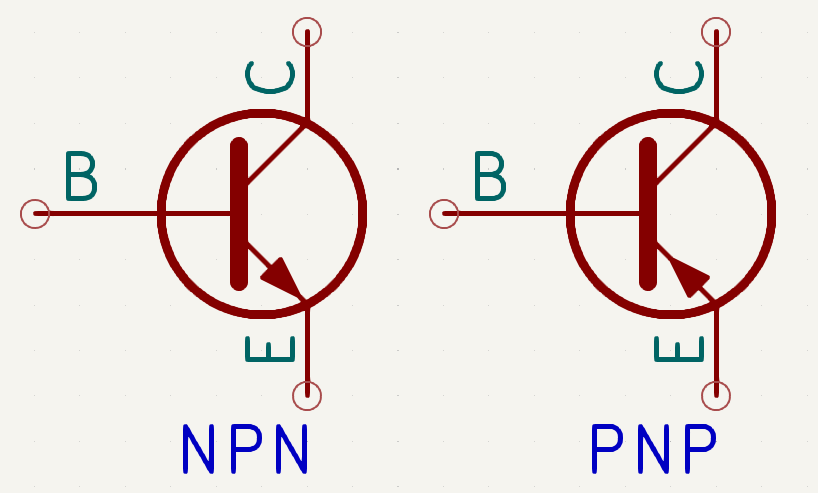
\includegraphics[width=0.8\textwidth]{graphit/bjt_circuit.png}
        \caption{BJTの回路記号}
        \label{fig:bjt_cir}
    \end{minipage}
    \begin{minipage}
        {0.3\hsize}
        \centering
        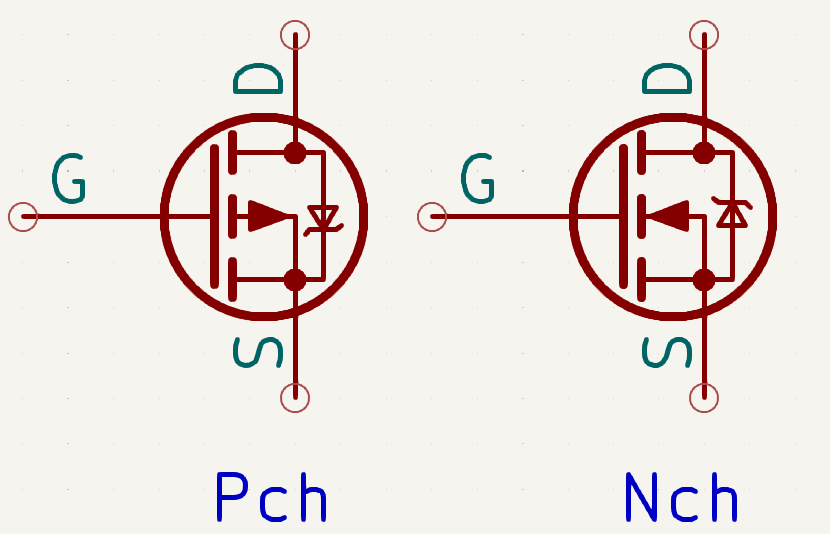
\includegraphics[width=0.8\textwidth]{graphit/mosfet_circuit.png}
        \caption{MOSFETの回路記号}
        \label{fig:mosfet_cir}
    \end{minipage}
\end{figure}
以下、この本ではこのように表記する。

各素子の論理回路での扱い方について説明する。
本来これらの素子は非線形素子であり、前章で習った基礎回路理論は通用しない。
しかし、論理回路では各素子をスイッチとして扱うことで、基礎回路理論を適用することができる。
\subsection{ダイオード}
ダイオードは順方向に電圧がかかると電流が流れ、逆方向に電圧がかかるとほとんど電流が流れない特性を持つ。
そのため、論理回路では順方向に閉じたスイッチ、逆方向に開いたスイッチとして扱う。
\subsection{バイポーラトランジスタ}
NPN型BJTはベースに十分な電流が流れるとコレクタからエミッタに大きな電流が流れ、ベースに電流が流れないとコレクタからエミッタにほとんど電流が流れない特性を持つ。
そのため、論理回路ではベースに電流が流れると導通し、ベースに電流が流れないととても大きい抵抗として扱う。

また、PNP型BJTは、ベースに負の電流が流れるとエミッタからコレクタに大きな電流が流れ、ベースに電流が流れないとエミッタからコレクタにほとんど電流が流れない特性を持つ。
そのため、論理回路ではベースに負の電流が流れると導通し、ベースに電流が流れないととても大きい抵抗として扱う。
\subsection{MOSFET}
Nch MOSFETはゲートソース間に十分な電圧がかかるとドレインからソースに大きな電流が流れ、ゲートソース間に電圧がかからないとドレインからソースにほとんど電流が流れない特性を持つ。
そのため、論理回路ではゲートソース間に電圧がかかると導通し、ゲートソース間に電圧がかからないととても大きい抵抗として扱う。

また、Pch MOSFETはゲートソース間に負の電圧がかかるとソースからドレインに大きな電流が流れ、ゲートソース間に電圧がかからないとソースからドレインにほとんど電流が流れない特性を持つ。
そのため、論理回路ではゲートソース間に負の電圧がかかると導通し、ゲートソース間に電圧がかからないととても大きい抵抗として扱う。%トランジスタ等素子の説明
% \input{chapters/column1.tex}%増幅回路
%トランジスタによる論理回路の実現
\chapter{論理回路の実装方法}

\section{簡単な論理回路の実現}
以下のBJTと抵抗を使った回路を考える。
\begin{figure}[htbp]
    \centering
    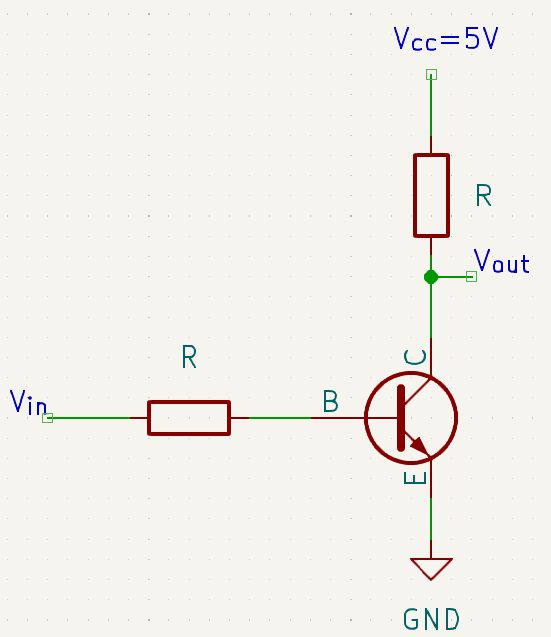
\includegraphics[width=0.3\textwidth]{BJT_logic/logic_circuit.png}
    \caption{}
    \label{fig:logic_circuit}
\end{figure}
この回路において$V_{in}$が0Vであるとき、BJTはベースに電流が流れないため、コレクタ-エミッタ間はとても大きい抵抗となり、$V_{cc}$からGNDに向かって電流が流れないため、
抵抗$R$による電圧降下が発生せず、出力電圧$V_{out}$は$V_{cc}$となる。
一方、$V_{in}$が5Vであるとき、BJTはベースに電流が流れるため、コレクタ-エミッタ間はショートとなり、抵抗$R$によりGNDに向かって電流が流れるため、
抵抗$R$による電圧降下が発生し、出力電圧$V_{out}$は0Vとなる。
以上より、0Vを論理0、5Vを論理1としたとき、以下の真理値表が得られる。
\begin{table}[htbp]
    \centering
    \begin{tabular}{|c|c|}
        \hline
        $V_{in}$ & $V_{out}$ \\
        \hline
        0V (論理0) & 5V (論理1) \\
        5V (論理1) & 0V (論理0) \\
        \hline
    \end{tabular}
    \caption{BJTを用いた論理回路の真理値表}
    \label{tab:logic_circuit_truth_table}
\end{table}
この真理値表はNOT回路の真理値表と一致するため、この回路はNOT回路として動作することがわかる。

ここで考えたいことがある。いま、0Vを論理0、5Vを論理1としたが、これは自明なのだろうか。
実は、0Vを論理1、5Vを論理0とすることも可能である。
電圧を高い状態をH,低い状態をLと表すと、
\begin{align}
  \left\{
    \begin{array}{l}
        L = 0 \\
        H = 1
    \end{array}
    \right.
\end{align}
とするか
\begin{align}
  \left\{
    \begin{array}{l}
        H = 0 \\
        L = 1
    \end{array}
    \right.
\end{align}
とするかの二種類がある。
前者を正論理、後者を負論理と呼ぶ。
この本では、特に断りがない限り正論理を採用する。

とにかく、図\ref{fig:logic_circuit}の回路はNOT回路として動作することがわかった。
また、AND回路やOR回路も図\ref{fig:and_circuit}、図\ref{fig:or_circuit}のようにBJTと抵抗を組み合わせることで実現できる。
\begin{figure}[htbp]
    \begin{minipage}
        {0.45\hsize}
        \centering
        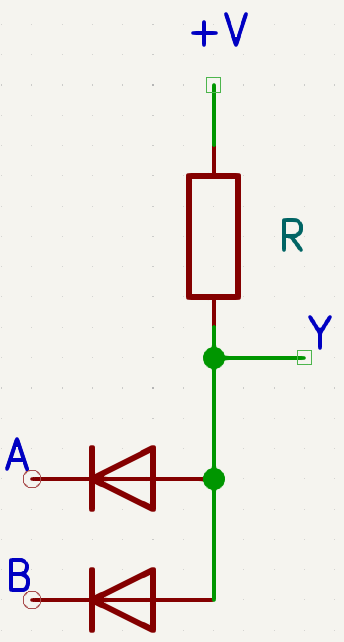
\includegraphics[width=0.4\textwidth]{BJT_logic/and_circuit.png}
        \caption{AND回路}
        \label{fig:and_circuit}
    \end{minipage}
    \begin{minipage}
        {0.45\hsize}
        \centering
        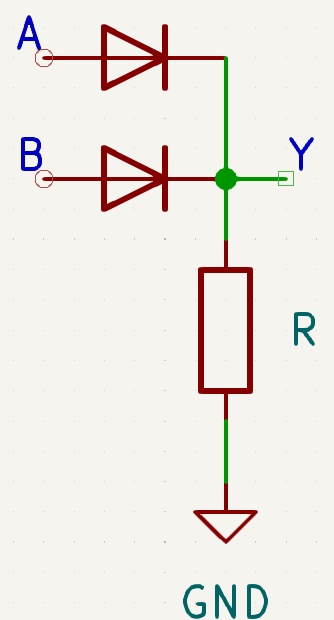
\includegraphics[width=0.4\textwidth]{BJT_logic/or_circuit.png}
        \caption{OR回路}
        \label{fig:or_circuit}
    \end{minipage}
\end{figure}

まず、図\ref{fig:and_circuit}のAND回路について説明する。
AとBの両方が+Vであるとき、ダイオードは導通せず電流は流れないため、抵抗$R$による電圧降下が発生せず、出力電圧$V_{out}$は$V_{cc}$となる。
一方、AまたはBのいずれかが0Vであるとき、対応するダイオードが順方向に導通し、抵抗$R$により0Vの入力に向かって電流が流れるため、抵抗$R$による電圧降下が発生し、出力電圧$V_{out}$は0Vとなる。
よってAND回路の真理値表が得られる。

次に、図\ref{fig:or_circuit}のOR回路について説明する。
AまたはBのいずれかが+Vであるとき、対応するダイオードが順方向に導通し、抵抗$R$によりGNDに向かって電流が流れるため、抵抗$R$による電圧降下が発生し、出力電圧$V_{out}$は$V_{cc}$となる。
一方、AとBの両方が0Vであるとき、ダイオードは導通せず電流は流れないため、抵抗$R$による電圧降下が発生せず、出力電圧$V_{out}$は0Vとなる。
よってOR回路の真理値表が得られる。

しかし、これらの回路には問題点がある。
先ほどまでは無視していたが実際には、ダイオードには空乏層分の電圧降下が存在する。
まずAND回路のほうであるが、Y=Lのとき、ダイオードの空乏層分の電圧が発生してしまうため、Yの電圧が完全に0Vにならない。
次にOR回路のほうであるが、Y=Hのとき、出力電圧がダイオードの空乏層分の電圧だけ低くなってしまうため、Yの電圧が完全に$V_{cc}$にならない。
また、共通の問題として、抵抗に電流が流れ続けるため、電力消費が大きいという問題、負荷によって出力電圧が変動してしまうという問題がある。
よって、現在では、これらの回路はあまり使われておらず、より優れた回路が使われている。



\section{バイポーラトランジスタによる論理回路の実現}

前部の回路の問題点として、出力電圧が完全に0Vまたは$V_{cc}$にならないこと、電力消費が大きいこと、大電流が扱えないこと、
出力インピーダンスが高く負荷によって出力電圧が変動してしまう、入力インピーダンスが低いことが挙げられた。

ひとつづつこれらの問題点を解決していこう。
まず、入力インピーダンスが低いという問題についてであるが、BJTをスイッチとして使うことで解決できる。
図\ref{fig:bjt_logic_circuit}にBJTを用いたNAND回路を示す。
\begin{figure}[htbp]
    \centering
    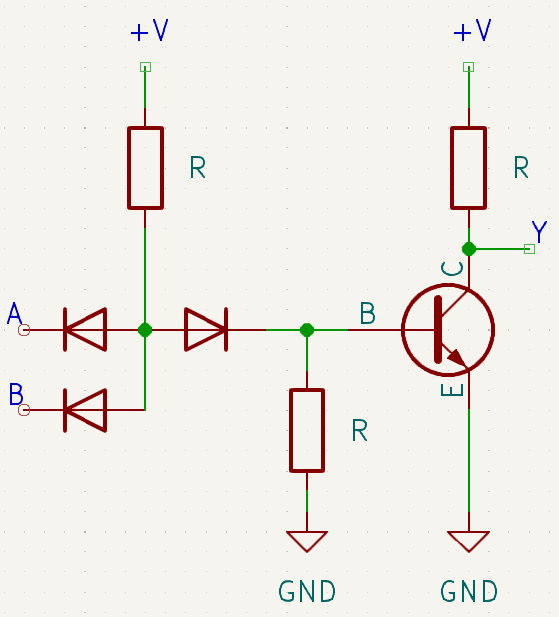
\includegraphics[width=0.3\textwidth]{BJT_logic/bjt_logic_circuit.png}
    \caption{BJTを用いたNAND回路}
    \label{fig:bjt_logic_circuit}
\end{figure}
この回路のようにダイオードとBJTを組み合わせた論理回路のことをダイオード-トランジスタ論理(DTL: Diode-Transistor Logic)回路と呼ぶ。
この回路は前の章のAND回路に反転増幅回路を組み合わせたものであるため、NAND回路として動作することが分かる。
これによって入力インピーダンスの問題に加え、出力電圧が0Vまたは$V_{cc}$にならない問題が解決できた。

次に、大電流が扱えないという問題についてであるが、ダイオードの代わりにBJTを使うことで解決できる。
前章のBJTの理論で余談として述べたが、BJTのベースエミッタ間はダイオードと同様の電流-電圧特性を持つため、ダイオードの代わりにBJTを使うことで大電流を扱うことができる。
トランジスタの量を増やすことに不満があるかもしれないが、結局現在では集積回路としてIC化されているため、ダイオードもトランジスタももはや変わらず、
高速動作性や大電流化のためにBJTを使うことが多い。
ダイオードの代わりにBJTを使う論理回路のことをトランジスタ-トランジスタ論理(TTL: Transistor-Transistor Logic)回路と呼ぶ。

残りの問題は出力インピーダンスと電力消費であるが、これらは出力部に抵抗がついていることが原因である。
この抵抗を取り除き、出力段にトーテムポール回路を採用することで解決できる。

図\ref{fig:ttl_totem_pole}にBJT回路による、TTLトーテムポール出力を有したNAND回路を示す。
\begin{figure}[htbp]
    \centering
    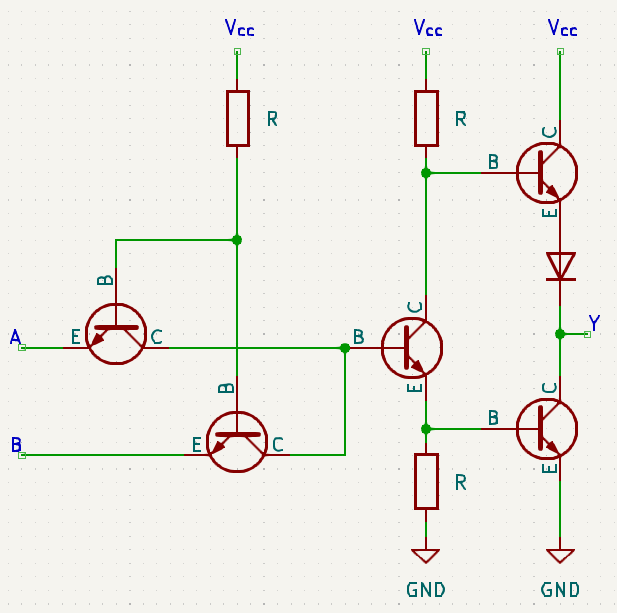
\includegraphics[width=0.5\textwidth]{BJT_logic/ttl_totem_pole.png}
    \caption{TTLトーテムポール出力を有したNAND回路}
    \label{fig:ttl_totem_pole}
\end{figure}

\newpage


この回路の動作を考えよう。
まず、AとBのどちらかが0Vであるとき、対応する入力部のトランジスタがonとなるため、
増幅部(2段目)のトランジスタがoffとなり、出力部(3段目)の上側のトランジスタがon、下側のトランジスタがoffとなる。
そのため、出力電圧$V_{out}$は$V_{cc}$からダイオードの順方向電圧降下分を引いた電圧となる。
一方、AとBの両方が+Vであるとき、入力部のトランジスタがどちらもoffとなるため、
増幅部のトランジスタがonとなり、出力部の上側のトランジスタがoff、下側のトランジスタがonとなる。
そのため、出力電圧$V_{out}$は0Vとなる。
以上より、この回路はNAND回路として動作することが分かる。
これによって出力電圧が完全に0Vまたは$V_{cc}$にならない問題以外の問題は解決できた。
これでNAND回路の実現方法について説明したが、AND回路やOR回路も同様にして実現できる。

また、余談ではあるが、このままの回路であると、出力部の上側と下側のトランジスタが同時にonとなる可能性があり、その瞬間$V_{cc}$からGNDに向かって大電流(貫通電流)が流れてしまう。
これを防ぐために、出力部の上側のトランジスタのコレクタ側に小さめの抵抗(130$\Omega$程度)を挿入することが多い。

以上より、BJTを用いた論理回路の実現方法について説明した。
しかし実は現在では、BJTを用いた論理回路はあまり使われておらず、MOSFETを用いた論理回路が主流となっている。
次章ではMOSFETを用いた論理回路の実現方法について説明する。

%トランジスタによる論理回路の実現
%MOSFETによる論理回路の実現
\section{MOSFETによる論理回路の実現}
前章ではBJTを用いた論理回路の実現方法について説明したが、現在ではMOSFETを用いた論理回路が主流となっている。
\newpage
図\ref{fig:mosfet_not}の回路を考えよう。
\begin{figure}[htbp]
    \begin{minipage}{0.35\hsize}
        \centering
        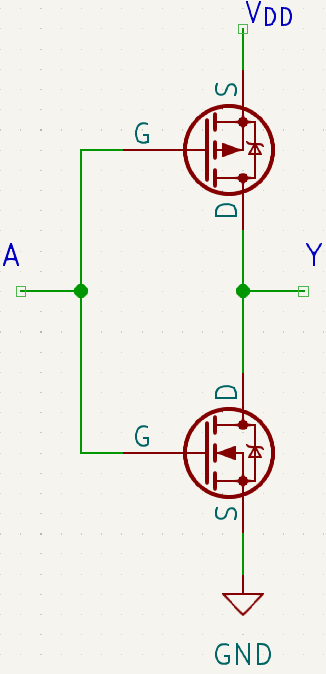
\includegraphics[width=0.5\textwidth]{MOSFET_logic/mosfet_not.png}
        \caption{MOSFETを用いたNOT回路}
        \label{fig:mosfet_not}
    \end{minipage}
    \begin{minipage}{0.55\hsize}
        \centering
        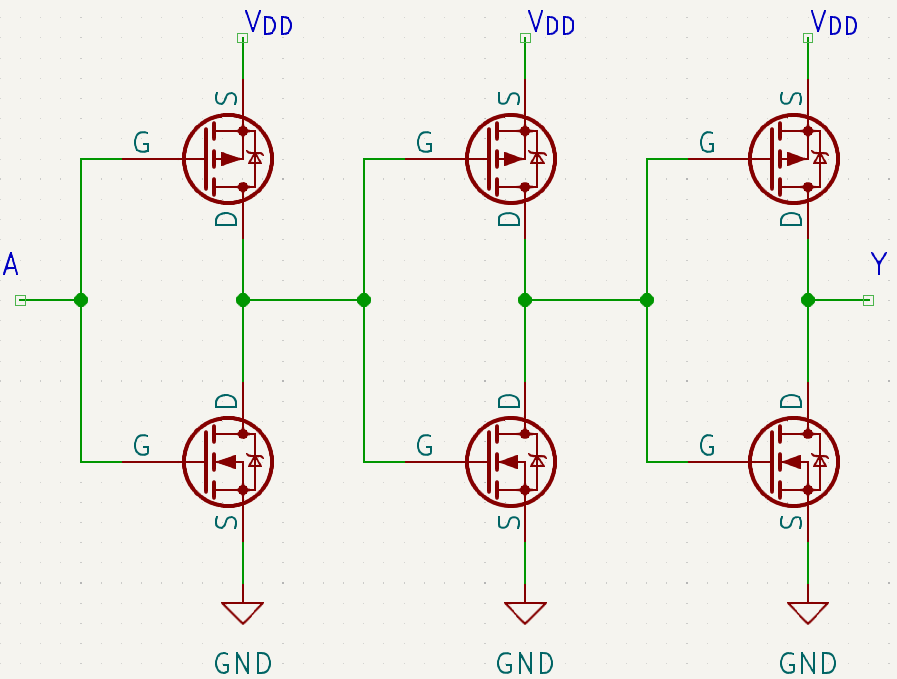
\includegraphics[width=0.9\textwidth]{MOSFET_logic/mosfet_not_real.png}
        \caption{実際のCMOSによるNOT回路}
        \label{fig:mosfet_not_real}
    \end{minipage}

\end{figure}

この回路は、PMOSトランジスタとNMOSトランジスタを組み合わせた回路であり、Complementary MOS (CMOS) 回路と呼ばれる。
復習であるが,Nch MOSFETはゲートにソースより高い電圧が印加されるとオンになる特性を持ち、Pch MOSFETはゲートにソースより低い電圧が印加されるとオンになる特性を持つ。
この回路において、入力が高電位（論理1）の場合、下側のNMOSトランジスタがオンになり、上側にPMOSトランジスタがオフになるため、出力はグランドに接続され、低電位（論理0）となる。
一方、入力が低電位（論理0）の場合、上側のPMOSトランジスタがオンになり、下側のNMOSトランジスタがオフになるため、出力は電源に接続され、高電位（論理1）となる。
このように、図\ref{fig:mosfet_not}の回路はNOT回路として動作する。

このCMOS回路の利点として、MOSFETを使用しているため、入力にほとんど電流が流れないため、入力インピーダンスが非常に高いことが挙げられる。
また、出力インピーダンスも低いため、他の回路への駆動能力が高い。
一方で、デメリットとして、MOSFETのゲートに電荷をチャージする時間だけ遅延が発生するため、スイッチング速度がBJTに比べて遅いこと、
静電気に弱いため、取り扱いに注意が必要であること、ONからOFFへの遷移時に一瞬両方のMOSFETがオンになるため、短時間ながらも電源からグランドに大きな電流が流れることが挙げられる。

なお実際のCMOSによるNOT回路では、図\ref{fig:mosfet_not_real}のように、図\ref{fig:mosfet_not}の回路を3個つなげて使っていることが多い。
% \begin{figure}[htbp]
%     \centering
%     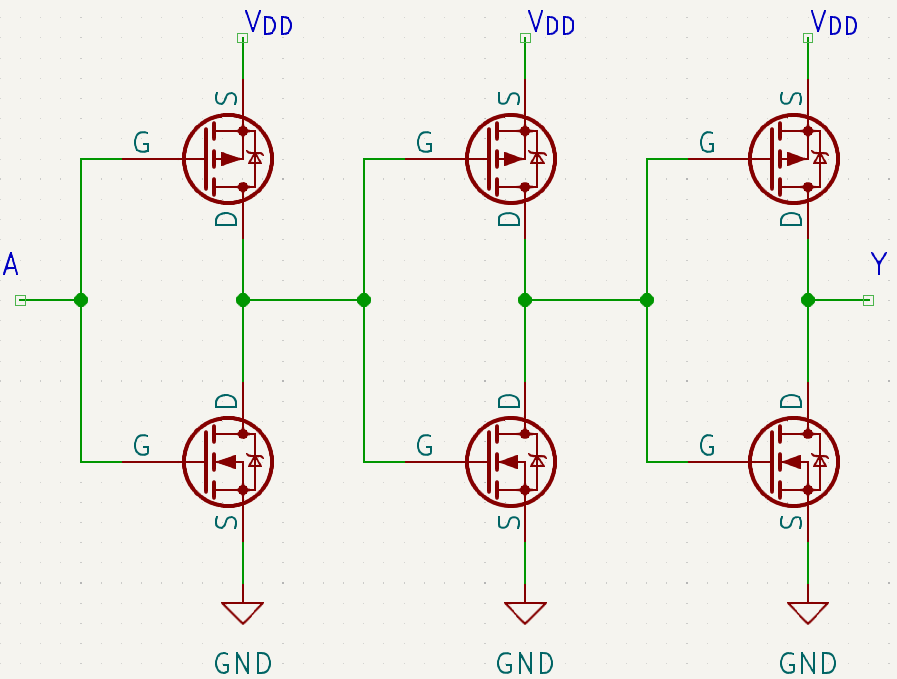
\includegraphics[width=0.5\textwidth]{MOSFET_logic/mosfet_not_real.png}
%     \caption{実際のCMOSによるNOT回路}
%     \label{fig:mosfet_not_real}
% \end{figure}

まず、図\ref{fig:mosfet_not}の回路はNOT回路を3つ直列につなげているため、出力もNOT回路となることがわかる。
これは、NOT回路の遅延時間等の特性をほかの論理回路と合わせるためであり、このような処理をした出力をバッファード出力と呼ぶ。

\newpage

次に、図\ref{fig:mosfet_nand}の回路を考えよう。
\begin{figure}[htbp]
    \centering
    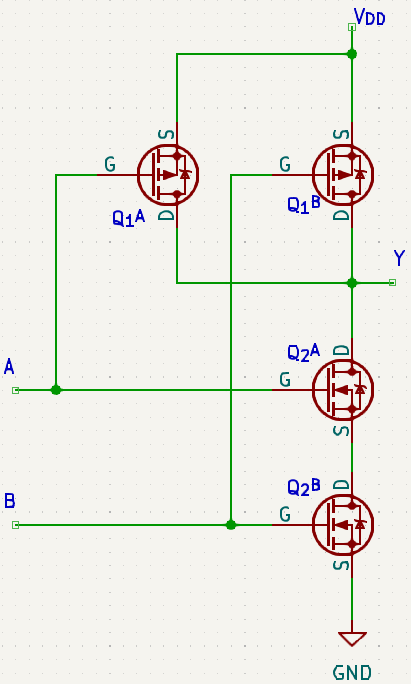
\includegraphics[width=0.4\textwidth]{MOSFET_logic/mosfet_nand.png}
    \caption{MOSFETを用いたNAND回路}
    \label{fig:mosfet_nand}
\end{figure}
この回路は、2つのPMOSトランジスタと2つのNMOSトランジスタを組み合わせた回路であり、NAND回路として動作する。
動作を確認しよう。
まず、入力Aが低電位(L)で、入力Bが低電位(L)の場合、$Q_1^A$と$Q_1^B$がオンになり、$Q_2^A$と$Q_2^B$がオフになるため、出力は電源に接続され、高電位(H)となる。
次に、入力Aが低電位(L)で、入力Bが高電位(H)の場合、$Q_1^A$と$Q_2^B$がオンになり、$Q_1^B$と$Q_2^A$がオフになるため、出力は電源に接続され、高電位(H)となる。
同様に、入力Aが高電位(H)で、入力Bが低電位(L)の場合も、出力は高電位(H)となる。
最後に、入力Aが高電位(H)で、入力Bが高電位(H)の場合、$Q_2^A$と$Q_2^B$がオンになり、$Q_1^A$と$Q_1^B$がオフになるため、出力はグランドに接続され、低電位(L)となる。
このように、図\ref{fig:mosfet_nand}の回路はNAND回路として動作する。

AND回路はNAND回路の出力をNOT回路(図\ref{fig:mosfet_not})に入力することで実現できるほか、NOR回路やOR回路も同様にして実現できる。
図\ref{fig:mosfet_all}の回路はそれぞれNOT回路、NAND回路、AND回路、NOR回路、OR回路をMOSFETで実現したものである。
特に動作原理を解説することはしないが、NAND回路の時と同じ考えで動作原理を確認することができるので、各自で確認してほしい.

\begin{figure}[htbp]
    \centering
    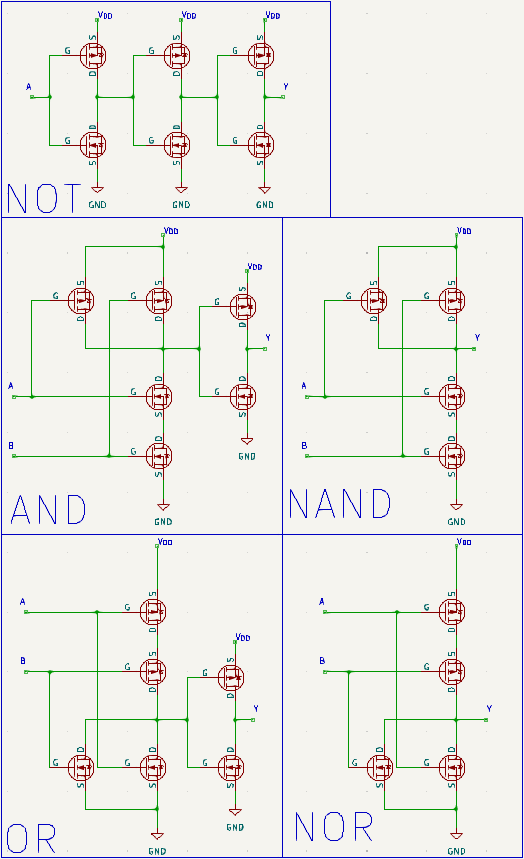
\includegraphics[width=0.95\textwidth]{MOSFET_logic/mosfet_all.png}
    \caption{MOSFETを用いた各種論理回路}
    \label{fig:mosfet_all}
\end{figure}
\newpage

以上のように、MOSFETを用いた論理回路はBJTを用いた論理回路と同様に動作するが、MOSFETの特性を活かした高入力インピーダンスや低出力インピーダンス,
出力電圧が完全に0Vまたは$V_{DD}$になることなどの利点があるため、現在ではMOSFETを用いた論理回路が主流となっている。

一方で、大きな弱点として、静電気に弱いことが挙げられる。
MOSFETのゲートは非常に薄い酸化膜で覆われており、静電気によってこの酸化膜が破壊されると、MOSFETが正常に動作しなくなる可能性がある。
そのため、多くの論理ゲートには静電気防止用の回路が組み込まれている。(図\ref{fig:esd_protection})

\begin{figure}[htbp]
    \centering
    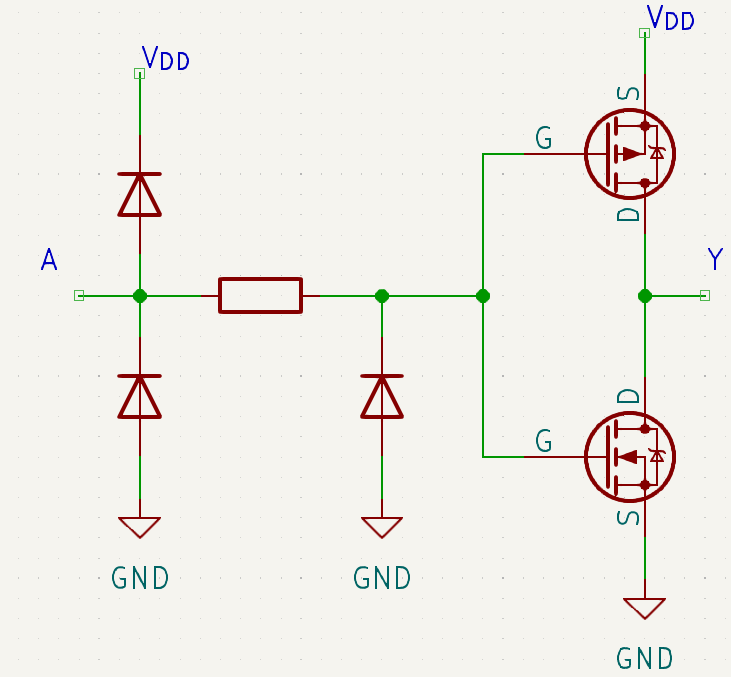
\includegraphics[width=0.5\textwidth]{MOSFET_logic/esd_protection.png}
    \caption{静電気防止回路の例}
    \label{fig:esd_protection}
\end{figure}

図\ref{fig:esd_protection}の回路では、入力端子に対して、$V_{DD}$とGNDにそれぞれダイオードが接続されている。
これにより、数万V程度にも及ぶ静電気が入力端子に加わった場合、電圧が正であっても負であってもダイオードが順方向に導通し、静電気を$V_{DD}$またはGNDに逃がすことで、MOSFETのゲートを保護している。
これで静電気によるMOSFETの破壊を防ぐことができるが、このダイオードは定常的に電流を流す設計になっていないので、
入力端子に$V_{DD}$より高い電圧を加えること、GNDより低い電圧を加えることは、論理回路の破壊の原因となるため、注意が必要である。

また、同様に、理論の章で説明したように、MOSFETには寄生ダイオードが存在するため、出力端子に$V_{DD}$より高い電圧を加えること、GNDより低い電圧を加えることも、論理回路の破壊の原因となるため、注意が必要である。


%MOSFETによる論理回路の実現
% %メカニカルリレーによる論理回路の実現
\section{メカニカルリレーによる論理回路の実現}


%リレーによる論理回路の実現
%オープンコレクタ出力について
% \section{オープンコレクタ出力}


%オープンコレクタ出力について
%電圧レベルの変換
\chapter{論理回路応用}
前章までで、論理回路の基本的な仕組みと作り方について説明した。
本章では、論理回路を実際に使用する際に必要となる応用的な知識について説明する。

\section{オープンコレクタ出力}
今まで、正論理として、論理0を低電位(L)、論理1を高電位(H)として説明してきた。
しかし、オープンコレクタ出力と呼ばれる出力形式では、論理0を低インピーダンス状態、論理1を高インピーダンス状態として扱う。
図\ref{fig:open_collector}の回路図を見てほしい。
\begin{figure}[htbp]
    \begin{minipage}
        {0.45\hsize}
        \centering
        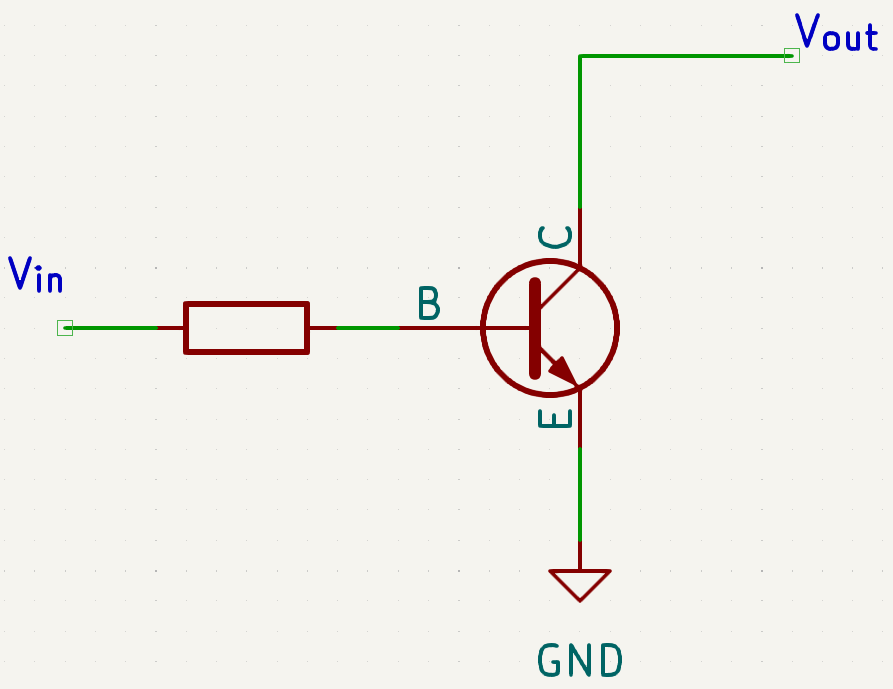
\includegraphics[width=0.8\textwidth]{apply/open_collector.png}
        \caption{出力回路}
        \label{fig:open_collector}
    \end{minipage}
    \begin{minipage}
        {0.45\hsize}
        \centering
        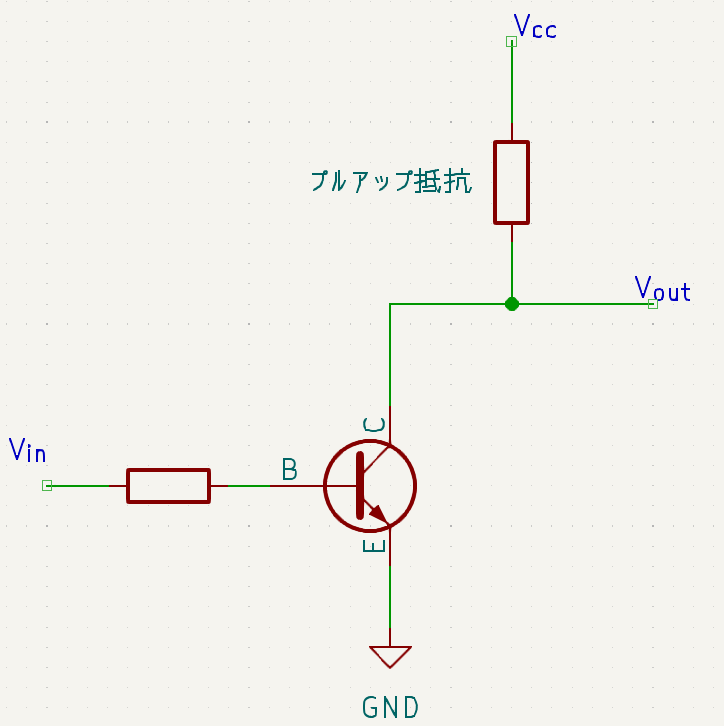
\includegraphics[width=0.8\textwidth]{apply/open_collector_pullup.png}
        \caption{プルアップ抵抗の接続}
        \label{fig:open_collector_pullup}
    \end{minipage}
\end{figure}
この回路は簡単なNOT回路からコレクタに接続されていた抵抗と電源を取り除いたものである。
この回路に$V_{in} = H$を入力すると、トランジスタがオンになるため、トランジスタはとても低い抵抗値とみなせるため、出力$V_{out}$はGNDにとても低い抵抗でつながっている状態となる。
これを低インピーダンス状態と呼ぶ。
一方、$V_{in} = L$を入力すると、トランジスタがオフになるため、トランジスタはとても高い抵抗値とみなせるため、出力$V_{out}$はGNDからとても高い抵抗でつながっている状態となる。
これを高インピーダンス状態と呼ぶ。
このようにオープンコレクタ出力では、論理0を低インピーダンス状態、論理1を高インピーダンス状態として扱う。

オープンコレクタ出力をそのまま扱うことはできないため、プルアップ抵抗と呼ばれる抵抗を出力に接続して使用する。(図\ref{fig:open_collector_pullup}参照)
この回路の動作は、

- $V_{in} = H$の場合、電源→プルアップ抵抗→出力→トランジスタ→GNDの経路ができ、トランジスタが低インピーダンス状態であるため、分圧により出力はGNDに近い低電位となる。(論理0)

- $V_{in} = L$の場合、電源→プルアップ抵抗→出力→トランジスタ→GNDの経路ができるが、トランジスタが高インピーダンス状態であるため、分圧により出力は電源に近い高電位となる。(論理1)

となる。
以上より、プルアップ抵抗とトランジスタの分圧比によって、出力の電圧レベルが決まるため、適切な抵抗値を選択する必要がある。

なおCMOS論理回路の場合、オープンドレイン出力と呼ばれることもあるが、基本的な動作は同じである。

この本ではオープンコレクタ出力を持つ論理回路は回路図上で、出力部に三角形のマークをつけて表記することにする。(図\ref{fig:open_collector_symbol}参照)
\begin{figure}[htbp]
    \centering
    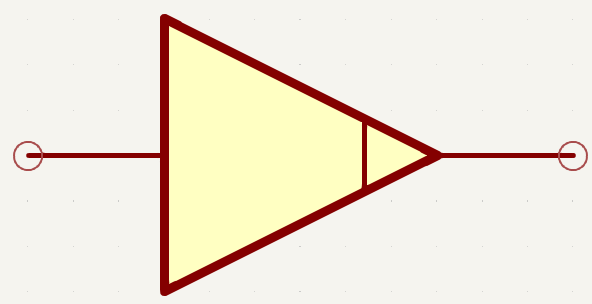
\includegraphics[width=0.2\textwidth]{apply/open_collector_symbol.png}
    \caption{オープンコレクタ出力のバッファ回路の記号}
    \label{fig:open_collector_symbol}
\end{figure}

ここで、オープンコレクタ出力の利点について説明しよう。
通常,各種論理出力をOR演算するときは、OR回路を使用する必要がある。(図\ref{fig:normal_or}参照)
一方で、オープンコレクタ出力の場合、複数の出力をそのまま接続して、プルアップするだけでOR演算が可能である。(図\ref{fig:open_collector_or}参照)
\begin{figure}[htbp]
    \begin{minipage}{0.45\hsize}
        \centering
        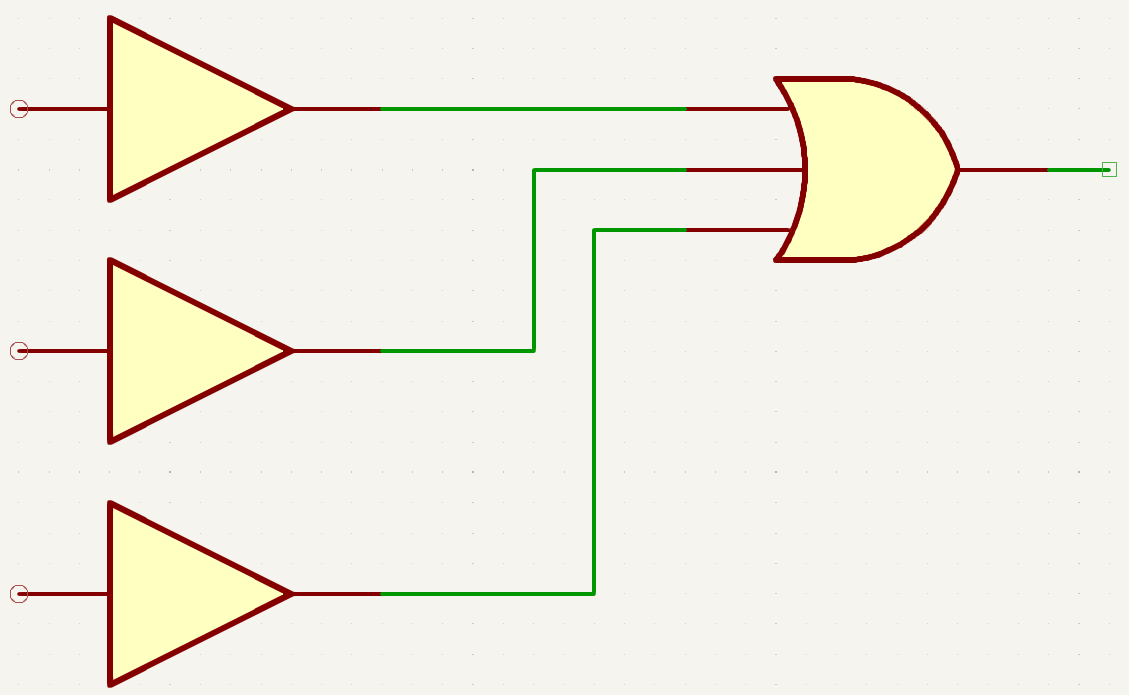
\includegraphics[width=0.6\textwidth]{apply/normal_or.png}
        \caption{通常のOR回路}
        \label{fig:normal_or}
    \end{minipage}
    \begin{minipage}{0.45\hsize}
        \centering
        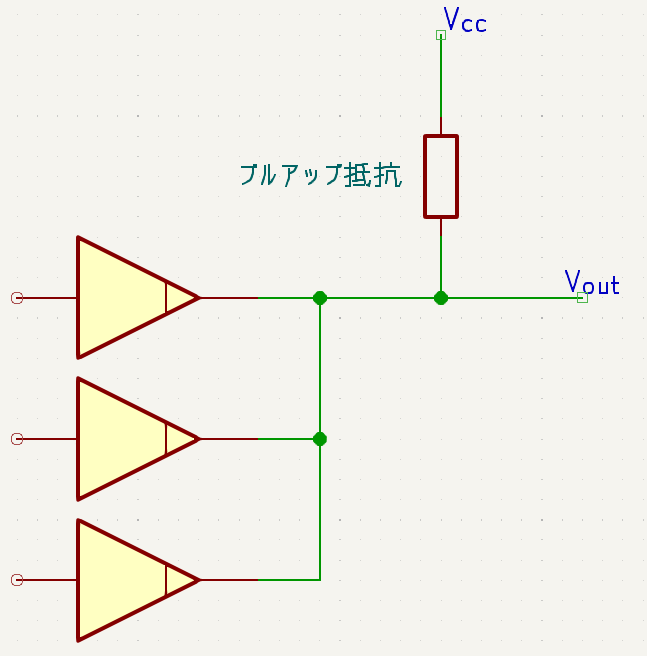
\includegraphics[width=0.6\textwidth]{apply/open_collector_or.png}
        \caption{オープンコレクタ出力によるOR回路}
        \label{fig:open_collector_or}
    \end{minipage}
\end{figure}

図\ref{fig:open_collector_or}の動作を確認しよう。
オープンコレクタ出力すべてが高インピーダンス状態の場合、プルアップ抵抗により出力は高電位(H)となる。
一方で、いずれか1つでも低インピーダンス状態、その部分を電流が通過するため、出力は低電位(L)となる。
このように、オープンコレクタ出力を使用することで、簡単に複数入力OR回路を実現できるという利点がある。これをワイアードORと呼ぶ。
なお負論理の場合は、オープンコレクタ出力を使用してAND回路を実現でき、ワイアードANDと呼ぶ。

このオープンコレクタ出力のTTLのNAND回路の回路図を図\ref{fig:ttl_open_collector_nand}に、オープンドレイン出力のCMOSのNAND回路の回路図を図\ref{fig:cmos_open_collector_nand}に示す。
\begin{figure}[htbp]
    \begin{minipage}{0.65\hsize}
        \centering
        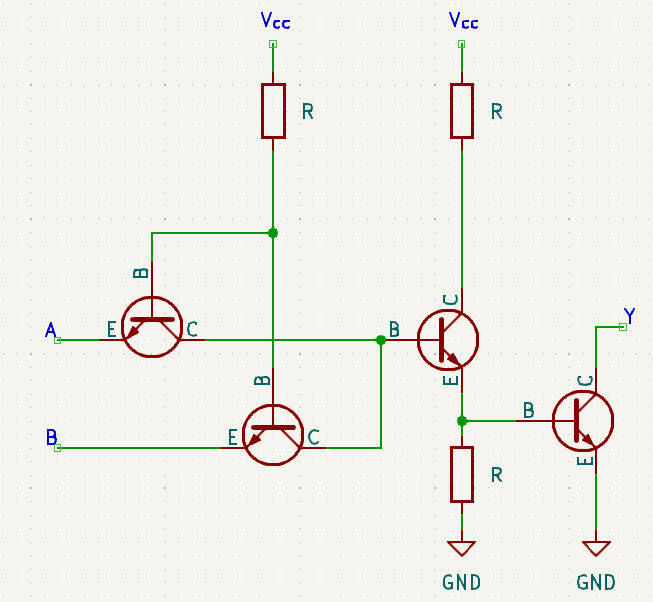
\includegraphics[width=0.8\textwidth]{apply/ttl_open_collector_nand.png}
        \caption{TTLオープンコレクタNAND回路}
        \label{fig:ttl_open_collector_nand}
    \end{minipage}
    \begin{minipage}{0.3\hsize}
        \centering
        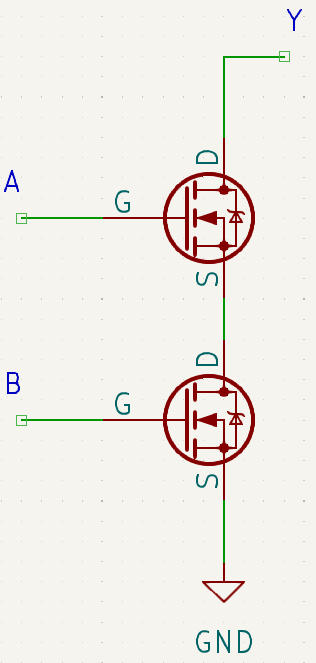
\includegraphics[width=0.8 \textwidth]{apply/cmos_open_collector_nand.png}
        \caption{CMOSオープンドレインNAND回路}
        \label{fig:cmos_open_collector_nand}
    \end{minipage}
\end{figure}

このようにオープンコレクタ出力を実装することができる。
NAND回路以外の論理回路でもオープンコレクタ出力を実装することができる。




\section{各種74シリーズ}
論理回路にはテキサス・インスツルメンツ社が開発した74シリーズと呼ばれるICが広く使われている。74シリーズには様々な種類があり、例えばTTLタイプの場合
\begin{itemize}
    \item 74シリーズ : 標準[standard] 
    \item 74Sシリーズ : 高速型[schottky]
    \item 74LSシリーズ : Sの低消費電力化[low power schottky]
    \item 74ALSシリーズ : LSの改良型[advanced low power schottky]
    \item 74ASシリーズ : Sの高速改良型[advanced schottky]
\end{itemize}
などがある。これらTTLタイプのものはほとんど絶滅しているが、74LSシリーズはまだ存在している。また、CMOSタイプの場合
\begin{itemize}
    \item 74Cシリーズ : CMOS標準[CMOS standard]
    \item 74HCシリーズ : 高速型[high speed CMOS]
    \item 74ACシリーズ : HCの改良型[advanced CMOS]
    \item 74AHCシリーズ : HCのさらなる改良型[advanced high speed CMOS]
    \item 74LVシリーズ : 3.3V以下の電源での動作[low voltage CMOS]
    \item 74LVCシリーズ : LVの高速型[advanced low voltage CMOS]
\end{itemize}
などがある。これらCMOSタイプのものは現在でも広く使われているが、特に74HCシリーズが主流である。

しかし、これらのICはそれぞれ違う電源電圧で動作したり、Hiであると認識する電圧レベルとHiとして出力する電圧レベルが異なったりするため(図\ref{fig:voltage_level})、
異なるシリーズのICを直接接続して使用することはできない。
\begin{figure}[htbp]
    \centering
    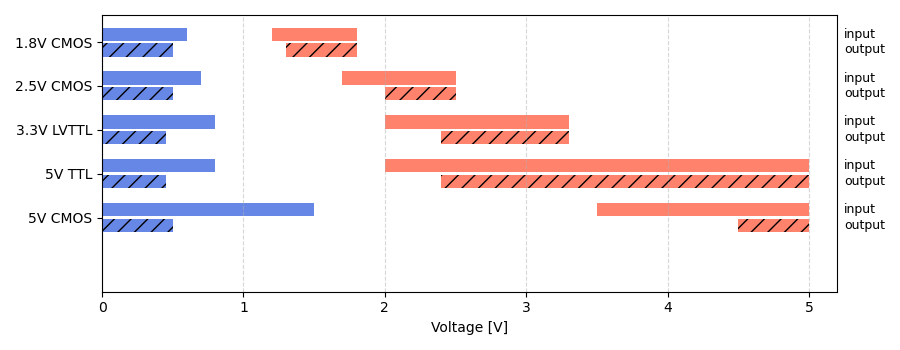
\includegraphics[width=0.95\textwidth]{apply/voltage_level.png}
    \caption{各種74シリーズの電圧レベル}
    \label{fig:voltage_level}
\end{figure}

しかし例外として、入出力トレラントと呼ばれる機能を持つICは、大きな電圧を入力や出力につないだ時でもICが壊れないように設計されているが、
動作は保障されていないので、異なる電圧レベルのIC同士を直接接続して使用するべきではない.

次の部では、異なる電圧レベルのIC同士を接続して使用する方法について説明する。

\section{電圧レベルの変換}

一口に電圧レベルが異なるといっても、出力レベルが入力レベルより高い場合の変換と、出力レベルが入力レベルより低い場合の変換の2種類がある。
まず、出力レベルが入力レベルより高い場合の変換について説明する。
\subsection{出力レベル>入力レベルの場合}
\subsubsection{抵抗分圧}
出力レベル>入力レベルの場合、まず考えることとして、抵抗分圧によって出力レベルを下げる方法がある。(図\ref{fig:voltage_divider}参照)
\begin{figure}[htbp]
    \centering
    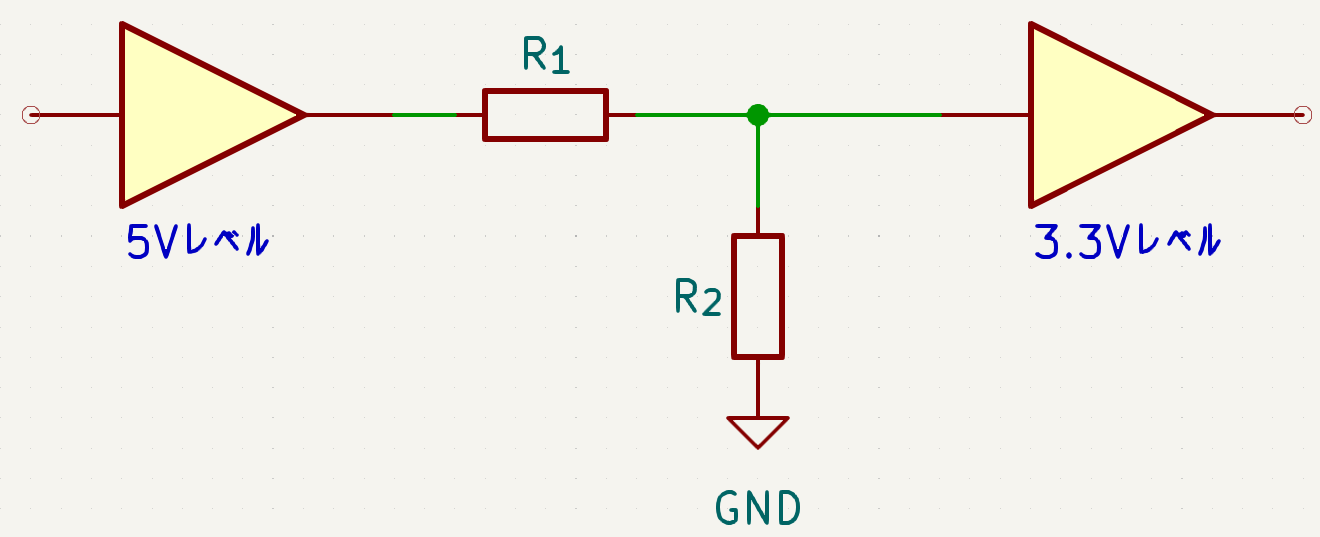
\includegraphics[width=0.5\textwidth]{apply/voltage_divider.png}
    \caption{抵抗分圧による電圧レベル変換}
    \label{fig:voltage_divider}
\end{figure}
この回路では、電圧レベルが5Vの出力を$R_1$と$R_2$の抵抗分圧によって、電圧レベルが3.3Vの入力に接続している。
このとき、
\begin{equation}
    V_{out} = V_{in} \cdot \frac{R_2}{R_1 + R_2}
\end{equation}
となるため、$R_1$と$R_2$の値を適切に選択することで、5Vの出力を3.3Vの入力に接続することができる。
しかし、この方法はゲートの出力がHighのとき、必ず$R_1$と$R_2$に電流が流れるため、消費電力が大きくなるという欠点がある。

また、アマチュアレベルでよく使われている方法として、単純に直列に抵抗を接続する方法がある。(図\ref{fig:series_resistor}参照)
\begin{figure}[htbp]
    \centering
    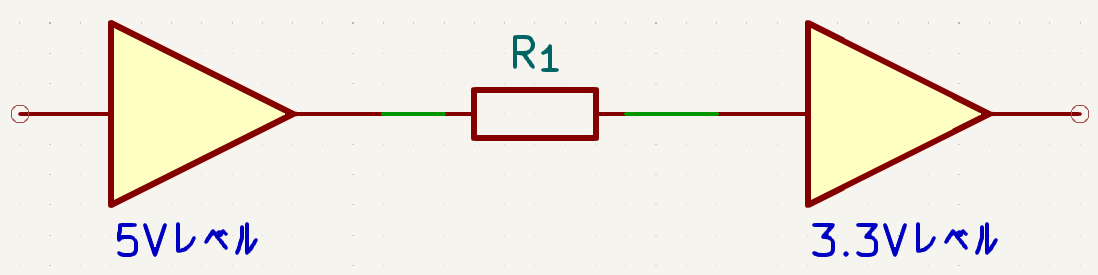
\includegraphics[width=0.5\textwidth]{apply/series_resistor.png}
    \caption{直列抵抗による電圧レベル変換}
    \label{fig:series_resistor}
\end{figure}

この回路は、5Vの出力と3.3Vの入力の間に直列に抵抗を接続している。
この回路は一応動作はするのだが、CMOSの静電気保護用のダイオードに電流が流れ続けるというメーカーの想定外の動作をするため、ICが壊れる可能性がある。(図\ref{fig:esd_diodes}参照)
\begin{figure}[htbp]
    \centering
    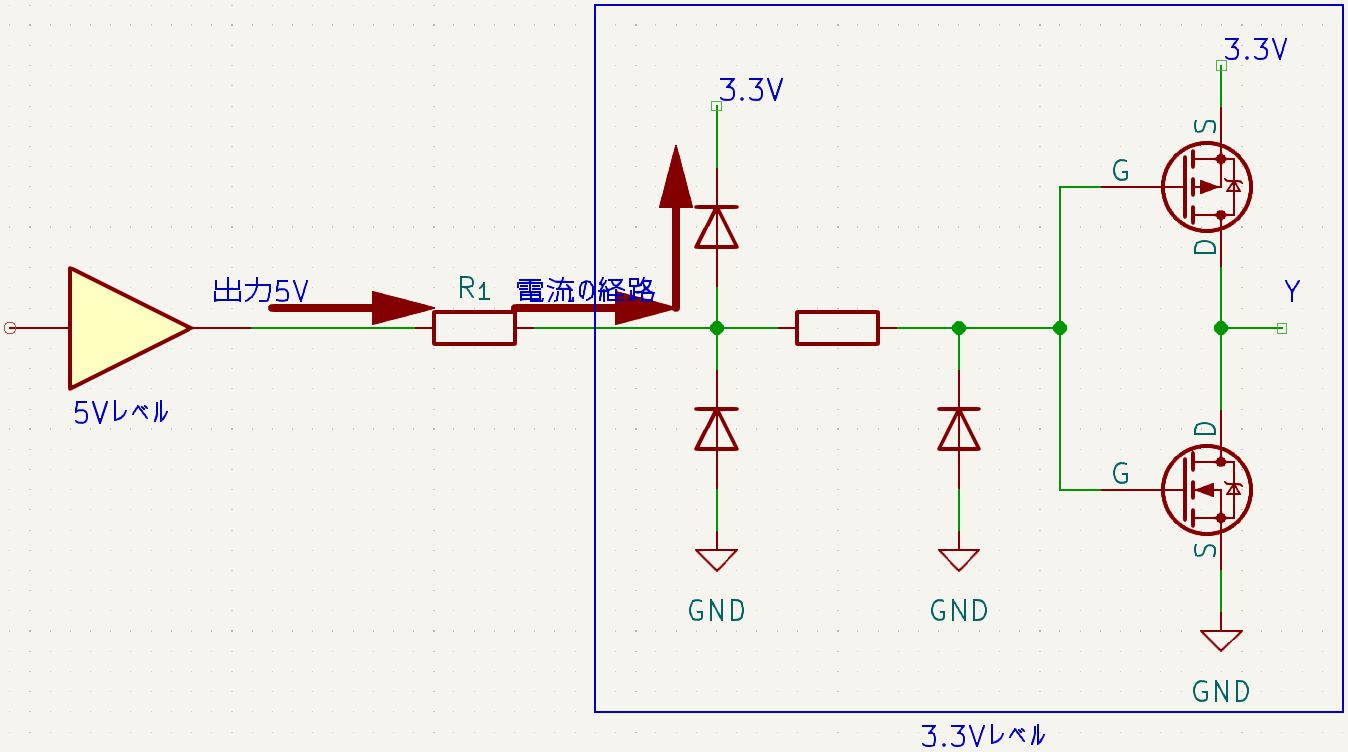
\includegraphics[width=0.5\textwidth]{apply/esd_diodes.png}
    \caption{CMOSの静電気保護用ダイオードに電流が流れ続ける様子}
    \label{fig:esd_diodes}
\end{figure}
そのため、この方法は推奨されない。

\newpage

\subsubsection{オープンコレクタ出力}
もう一つの方法として、オープンコレクタ出力を使用する方法がある。(図\ref{fig:open_collector_level_shift}参照)
\begin{figure}[htbp]
    \centering
    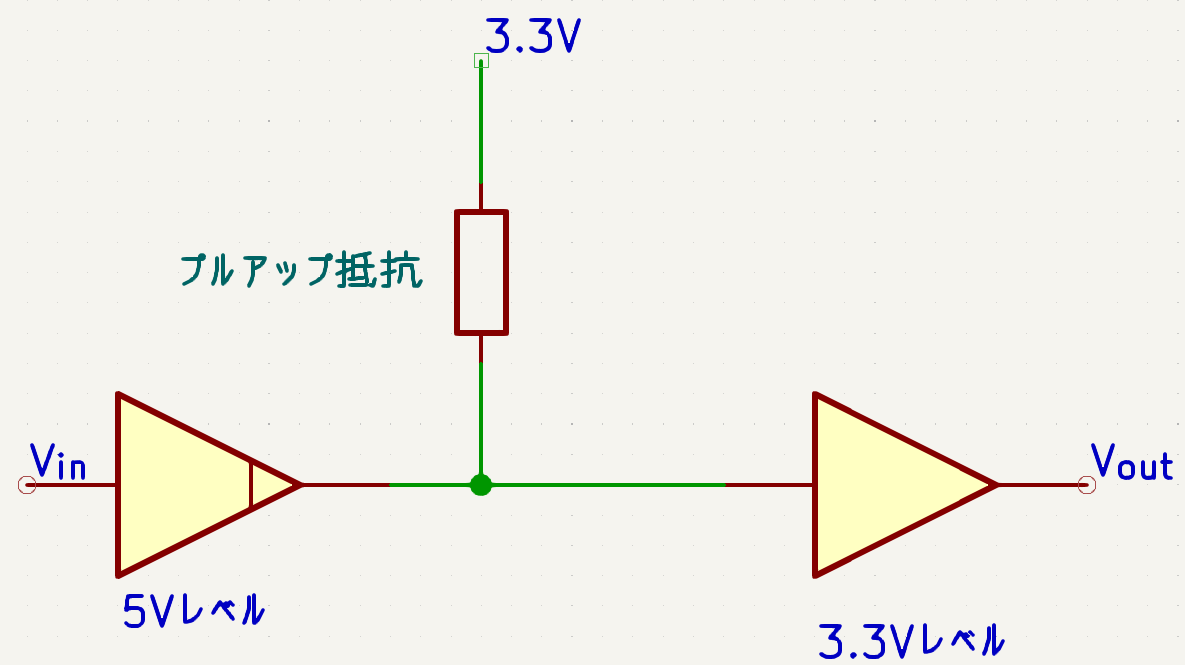
\includegraphics[width=0.5\textwidth]{apply/open_collector_level_shift.png}
    \caption{オープンコレクタ出力による電圧レベル変換}
    \label{fig:open_collector_level_shift}
\end{figure}

論理回路のレベルが5Vであったとしても、オープンコレクタ出力を使用することで、プルアップ抵抗の接続先を3.3Vにすることで、3.3Vの入力に接続することができる。

また、外部にトランジスタを用意することで、5V側がオープンコレクタ出力出なかったとしても、同様の理論でオープンコレクタ出力を実現することもできる。(図\ref{fig:transistor_open_collector}参照)
\begin{figure}[htbp]
    \centering
    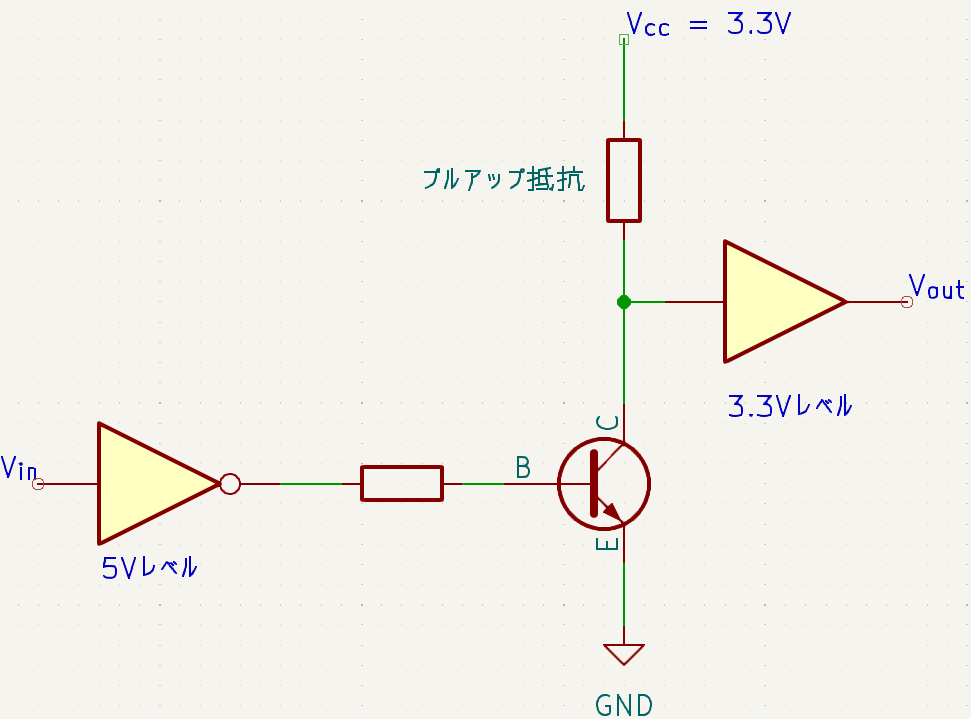
\includegraphics[width=0.5\textwidth]{apply/transistor_open_collector.png}
    \caption{トランジスタを用いたオープンコレクタ出力}
    \label{fig:transistor_open_collector}
\end{figure}

\subsubsection{レベル変換可能なゲートICを使う}
もう一つの方法として、レベル変換可能なゲートICを使用する方法がある。
レベル変換可能なゲートICとは、異なる電圧レベルで動作するデジタル回路間を安全に接続するために設計されたICであり、Texas Instruments社や東芝社などのメーカーから販売されている。
もし迷ったら、この方法を使用することが安全である。

\subsection{出力レベル<入力レベルの場合}
\subsubsection{そのままつなぐ}
出力レベル<入力レベルの場合、ほとんどの場合、そのまま接続しても論理回路が壊れることはない。
ここで、図\ref{fig:voltage_level}を見てほしいのであるが、3.3V LVTTLの出力と5V TTLの入力を接続した場合、
3.3V LVTTLの出力がHighのとき、出力は2.4V以上であるため、5V TTLの入力はHighとして認識する。
このように出力レベル<入力レベルの場合、そのまま接続しても問題ない場合が多い。

一方、3.3V LVTTLの出力と5V CMOSの入力を接続した場合を考えよう。
3.3V LVTTLの出力がHighのとき、出力は2.4V以上であるため、
5V CMOSの入力はHighとして認識する範囲の4.5Vに達しないため、
5V CMOSの入力はHighとして認識しない可能性がある.
この場合は別の方法を使用する必要がある。

\subsubsection{オープンコレクタ出力}
もう一つの方法として、オープンコレクタ出力を使用する方法がある。(図\ref{fig:open_collector_level_shift_low}参照)
\begin{figure}[htbp]
    \centering
    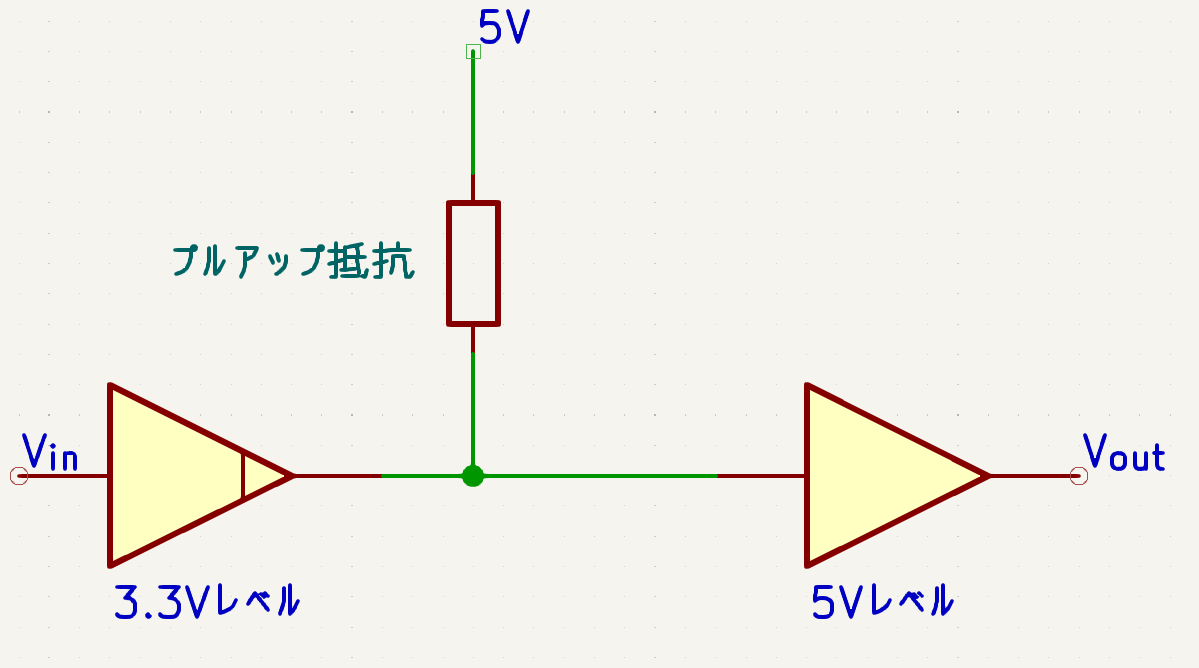
\includegraphics[width=0.5\textwidth]{apply/open_collector_level_shift_low.png}
    \caption{オープンコレクタ出力による電圧レベル変換(低電圧側入力)}
    \label{fig:open_collector_level_shift_low}
\end{figure}
論理回路のレベルが3.3Vであったとしても、オープンコレクタ出力を使用することで、プルアップ抵抗の接続先を5Vにすることで、5Vの入力に接続することができる。
しかし、注意点として、3.3V側の出力端子に5Vの電圧がかかるため、3.3V側のICには出力トレラント機能が必要である。

これもトランジスタを用意することで、5V側がオープンコレクタ出力出なかったとしても、同様の理論でオープンコレクタ出力を実現することもできる。

\subsubsection{レベル変換可能なゲートICを使う}
もう一つの方法として、前の節で紹介した、レベル変換可能なゲートICを使用する方法がある。
やはり、安全性などの観点から、この方法を使用することが推奨される。






%電圧レベル変換
%論理回路の入出力方法
\section{論理回路の入出力方法}

もしあなたが人間ならば、実際に電子工作で論理回路で何かを作成したときに、人間が論理回路に信号を与えてあげる入力と、人間が論理回路からの信号を受け取る出力が必要になるだろう。

\subsection{出力方法}
まず、論理回路の出力としてLEDを使うのが最もわかりやすい方法である。
A=HighのときにLEDが点灯し、A=LowのときにLEDが消灯するようにするには図\ref{fig:led_output_source}と図\ref{fig:led_output_sink}の2通りの方法がある。
\begin{figure}[htbp]
    \begin{minipage}
        {0.45\hsize}
        \centering
        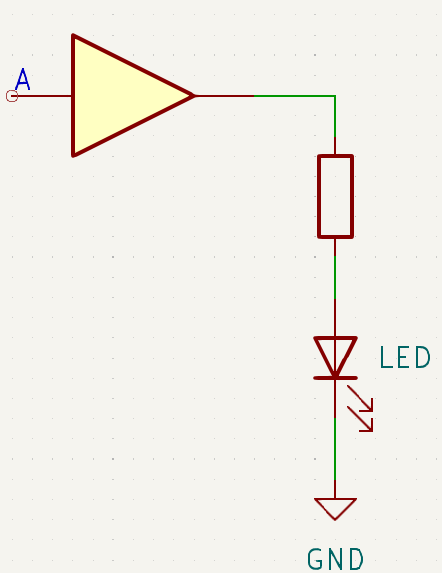
\includegraphics[width=0.6\textwidth]{apply/led_output_source.png}
        \caption{LEDをソース側に接続した出力回路}
        \label{fig:led_output_source}
    \end{minipage}
    \begin{minipage}
        {0.45\hsize}
        \centering
        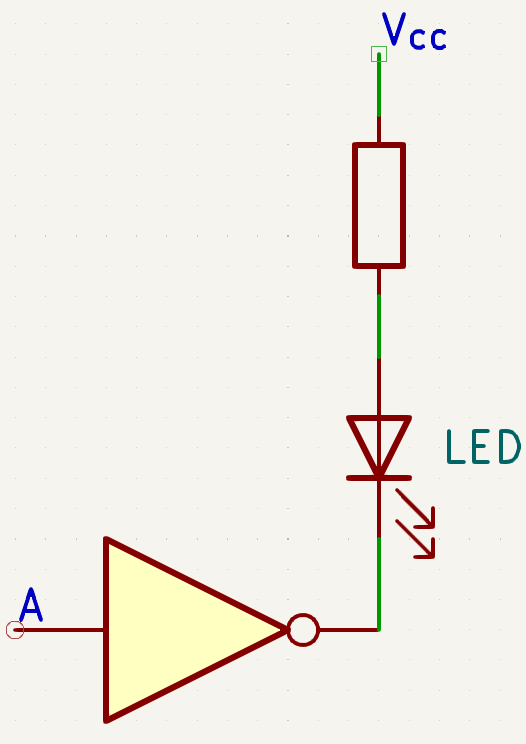
\includegraphics[width=0.6\textwidth]{apply/led_output_sink.png}
        \caption{LEDをシンク側に接続した出力回路}
        \label{fig:led_output_sink}
    \end{minipage}
\end{figure}
図\ref{fig:led_output_source}の回路では、論理回路の出力がHighのときに論理回路からLEDに電流が流れ、LEDが点灯する。
一方、図\ref{fig:led_output_sink}の回路では、論理回路の出力がLowのときに$V_{cc}$からLEDに電流が流れ、LEDが点灯する。
このように、どちらの方法でもLEDを点灯させることができる。

74HCシリーズの場合、論理回路が流せる電流は最大で約20mAであり、LEDが点灯するために必要な電流は約5～10mAであるため、直接LEDを接続しても問題ない。
しかし、LEDではない出力装置を使う場合や、複数のLEDを接続する場合などは、論理回路から直接電流を流すことができない場合がある。
その場合は、トランジスタを用いて論理回路の出力を増幅する必要がある。
図\ref{fig:transistor_output_emitter_ground},\ref{fig:transistor_output_emitter_follower}にトランジスタを用いた出力回路の例を示す。

\begin{figure}[htbp]
    \begin{minipage}
        {0.45\hsize}
        \centering
        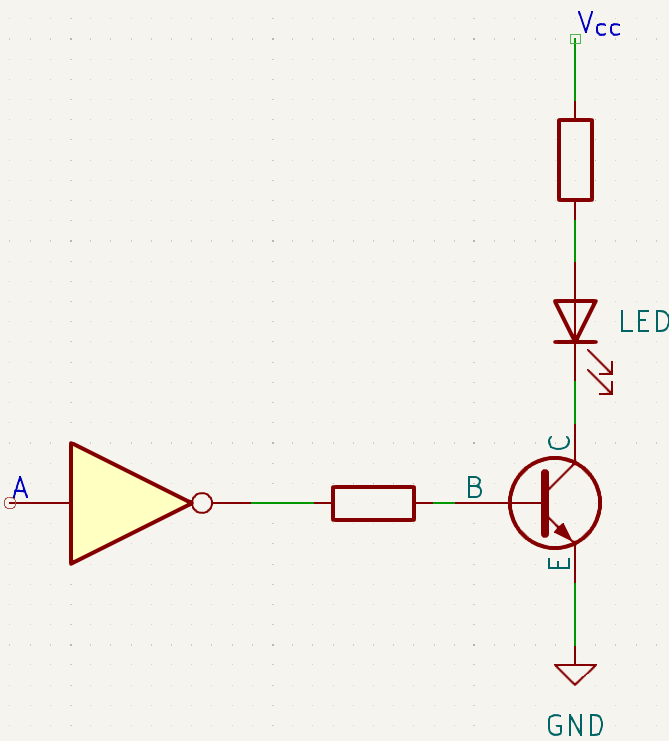
\includegraphics[width=0.8\textwidth]{apply/transistor_output_emitter_ground.png}
        \caption{エミッタ接地回路を用いた出力回路}
        \label{fig:transistor_output_emitter_ground}
    \end{minipage}
    \begin{minipage}
        {0.45\hsize}
        \centering
        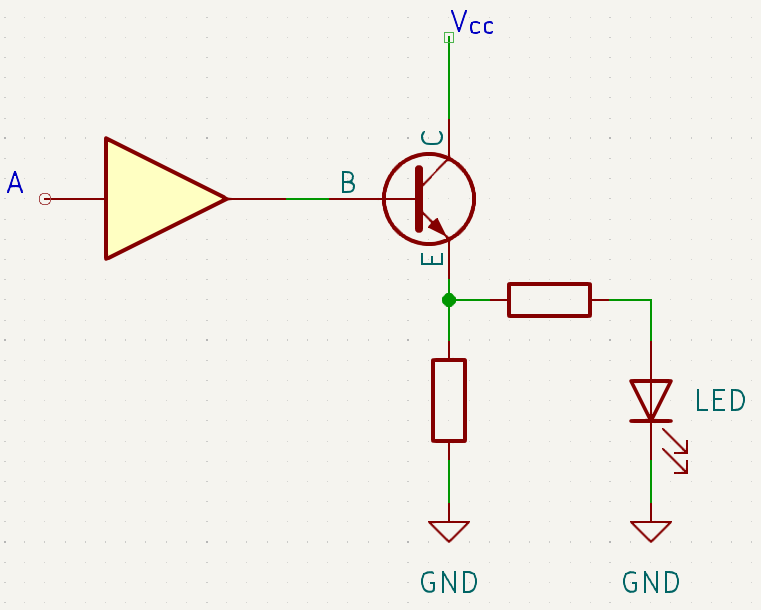
\includegraphics[width=0.95\textwidth]{apply/transistor_output_emitter_follower.png}
        \caption{エミッタフォロワ回路を用いた出力回路}
        \label{fig:transistor_output_emitter_follower}
    \end{minipage}
\end{figure}

\newpage

これらの回路を用いることで、論理回路の出力を増幅し、より大きな電流を流すことができる。

しかし、これらの回路には欠点が存在する。
トランジスタがONからOFFに切り替わるときに、トランジスタ内部に少数キャリアが過剰に残っているため、そいつらがキャリアとなり電流が流れなくなるまで時間がかかる。
この現象を少数キャリア蓄積効果と呼び、これによりスイッチング速度がおよそ3$\mu$s程度遅くなる。
このため、高速に動作させたい場合,図\ref{fig:transistor_output_emitter_ground_speedup}のような回路を用いる。
\begin{figure}[htbp]
    \centering
    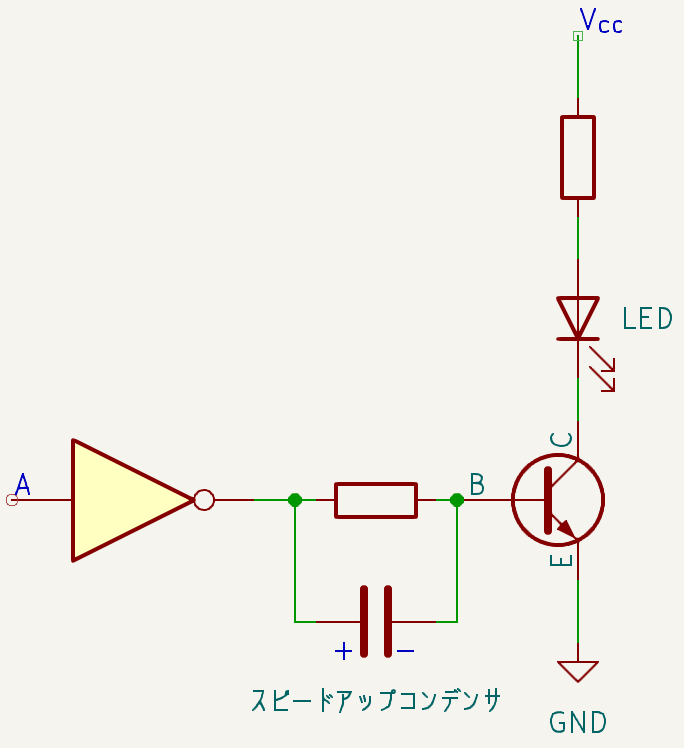
\includegraphics[width=0.5\textwidth]{apply/transistor_output_emitter_ground_speedup.png}
    \caption{スピードアップコンデンサを付けたエミッタ接地回路}
    \label{fig:transistor_output_emitter_ground_speedup}
\end{figure}
\newpage
この回路は100pF程度のコンデンサ(スピードアップコンデンサという)
を論理回路の出力とトランジスタのベースの間に接続することで、
論理回路の出力がHighの間に電荷を図の通りに蓄えて、Lowに切り替わったときに
その電荷を用いてベースに負の電圧をかけることで少数キャリアを強制的に排出し、スイッチング速度を向上させる回路である。

\subsection{入力方法}
論理回路に信号を入力する方法として、最も簡単な方法はスイッチを用いる方法である。
ここで図\ref{fig:switch_gate_fail1}のようにゲートにスイッチを接続したくなるが、この方法は正しく動作しない。
\begin{figure}[htbp]
    \begin{minipage}
        {0.45\hsize}
        \centering
        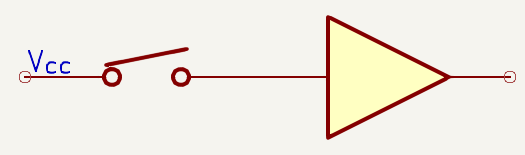
\includegraphics[width=0.6\textwidth]{apply/switch_gate_fail1.png}
        \caption{ゲートへのスイッチ接続例(誤1)}
        \label{fig:switch_gate_fail1}
    \end{minipage}
    \begin{minipage}
        {0.45\hsize}
        \centering
        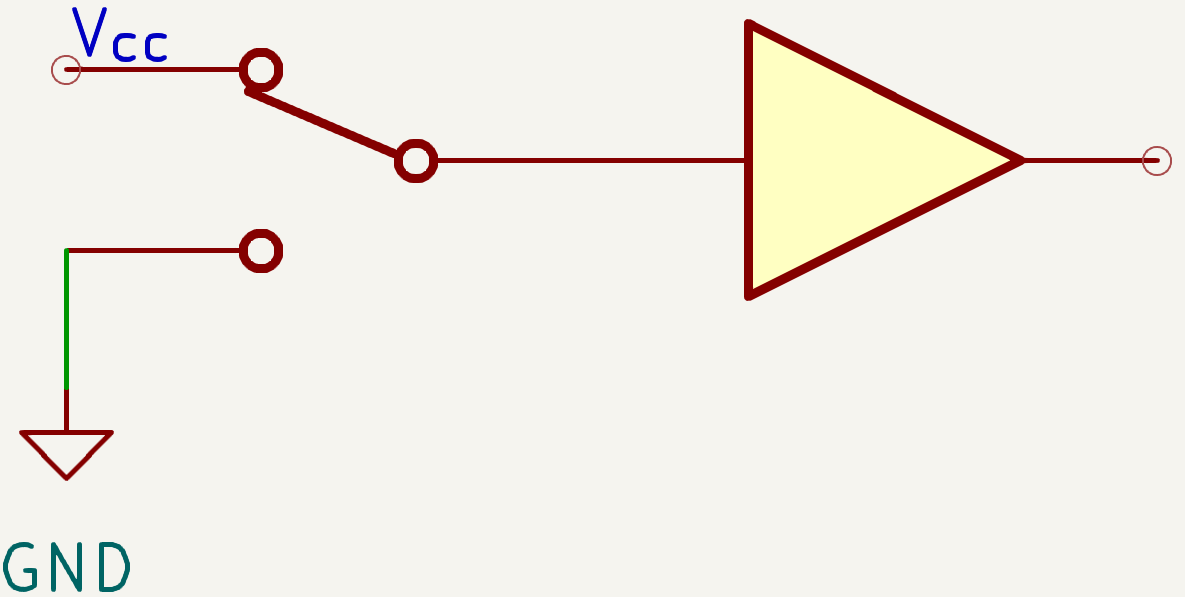
\includegraphics[width=0.6\textwidth]{apply/switch_gate_fail2.png}
        \caption{ゲートへのスイッチ接続例(誤2)}
        \label{fig:switch_gate_fail2}
    \end{minipage}
\end{figure}
なぜならば、このスイッチを開いた場合に、論理回路の入力が浮遊状態となり、不定の電圧となってしまうため、動作が保障されない。

図\ref{fig:switch_gate_fail1}の回路がだめならば、図\ref{fig:switch_gate_fail2}のようにスイッチでGNDと$V_{cc}$を切り替えればうまくいくかもしれないと考えるかもしれないが
、この方法も上手くいかない。
なぜならばスイッチはどちらかの接点と離れたタイミングと全く同じ時間にもう一つの接点と接続されるわけではないためである。
まず、切り替え時に両方の接点と離れてしまう場合(Break-Before-Makeという)、論理回路の入力が浮遊状態となり、不定の電圧となってしまうため、動作が保障されない。
一方、切り替え時に両方の接点と接続されてしまう場合(Make-Before-Breakという)、論理回路の入力が一瞬であるが短絡状態となってしまい、過大な電流が流れてしまう可能性があるため、危険である。
\newpage
このように、スイッチを用いて論理回路に信号を入力する場合は、プルアップ抵抗またはプルダウン抵抗を用いて、スイッチが開いたときに論理回路の入力が浮遊状態にならないようにする必要がある。
図\ref{fig:switch_gate_pullup}にプルアップ抵抗を用いたスイッチ接続例を、図\ref{fig:switch_gate_pulldown}にプルダウン抵抗を用いたスイッチ接続例を示す。
\begin{figure}[htbp]
    \begin{minipage}
        {0.45\hsize}
        \centering
        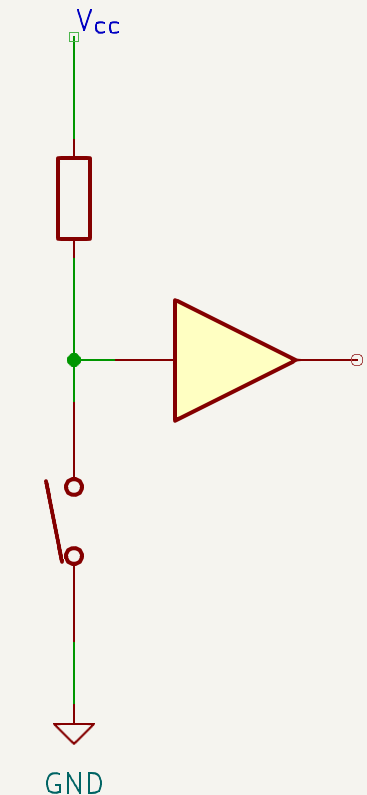
\includegraphics[width=0.6\textwidth]{apply/switch_gate_pullup.png}
        \caption{プルアップ抵抗を用いたゲートへのスイッチ接続例}
        \label{fig:switch_gate_pullup}
    \end{minipage}
    \begin{minipage}
        {0.45\hsize}
        \centering
        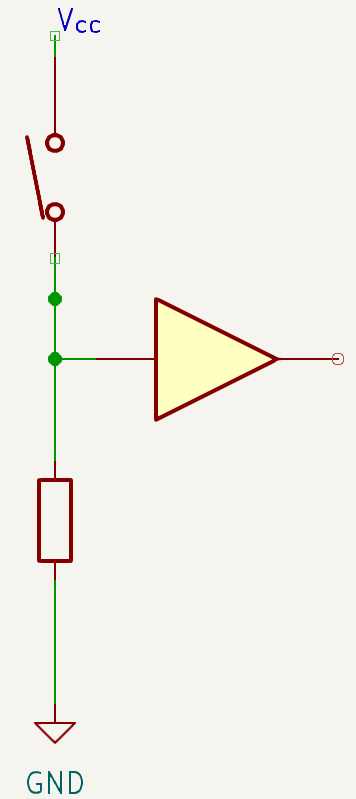
\includegraphics[width=0.6\textwidth]{apply/switch_gate_pulldown.png}
        \caption{プルダウン抵抗を用いたゲートへのスイッチ接続例}
        \label{fig:switch_gate_pulldown}
    \end{minipage}
\end{figure}
図\ref{fig:switch_gate_pullup}の回路では、スイッチが開いているときにプルアップ抵抗によって論理回路の入力が$V_{cc}$に引っ張られ、高電位(H)となる。
一方、スイッチが閉じているときに論理回路の入力がGNDに接続され、低電位(L)となる。
プルダウンの回路も同様に動作する。
このように、スイッチを用いて論理回路に信号を入力する場合は、プルアップ抵抗またはプルダウン抵抗を用いて、スイッチが開いたときに論理回路の入力が浮遊状態にならないようにする必要がある。

プルアップ、プルダウン抵抗の抵抗値は、通常数k$\Omega$から数十k$\Omega$程度が用いられる。

しかし、スイッチを使う際に注意しなければならない点がある。
スイッチを押したときに、接点がバウンドし、チャタリングと呼ばれる現象が発生することがある。
チャタリングが発生すると、スイッチを一回押しただけで、論理回路の入力がHighとLowを何度も繰り返すことになり、正しく動作しない可能性がある。
このチャタリングをはソフト的な対策を行うこともできるが、最も簡単なハード的対策として、図\ref{fig:switch_debounce}のようなチャタリング防止回路を用いることができる。
\begin{figure}[htbp]
    \begin{minipage}
        {0.45\hsize}
        \centering
        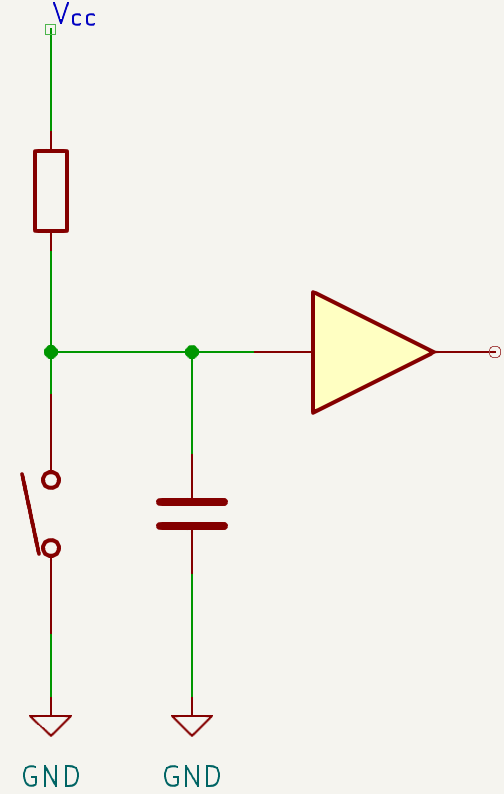
\includegraphics[width=0.7\textwidth]{apply/switch_debounce.png}
        \caption{チャタリング防止回路の例}
        \label{fig:switch_debounce}
    \end{minipage}
    \begin{minipage}
        {0.45\hsize}
        \centering
        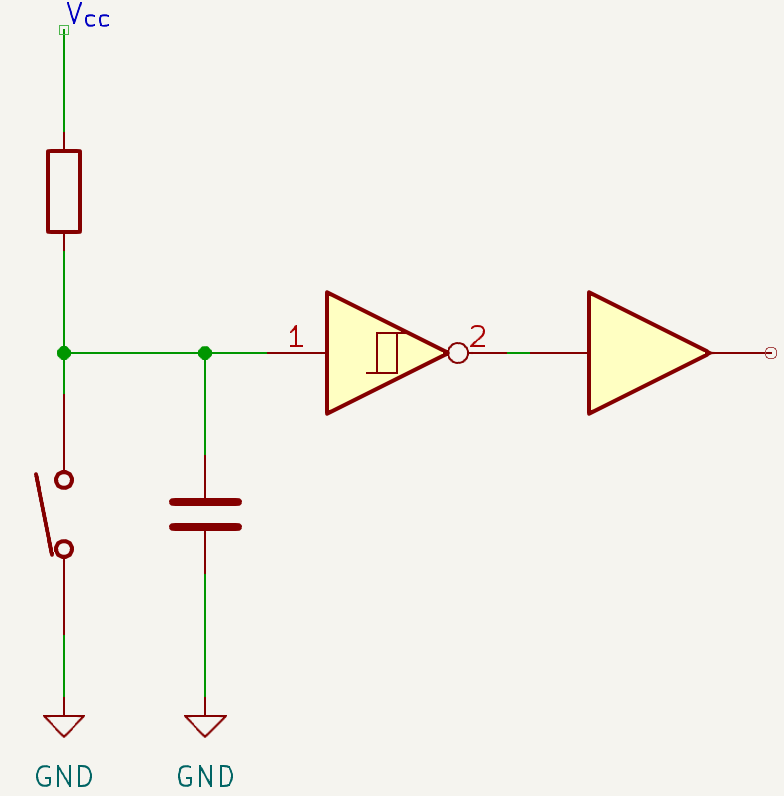
\includegraphics[width=0.9\textwidth]{apply/switch_debounce_schmitt.png}
        \caption{シュミットトリガ回路を組み合わせたチャタリング防止回路の例}
        \label{fig:switch_debounce_schmitt}
    \end{minipage}
\end{figure}

この回路ではチャタリングが発生しても、コンデンサ$C_1$が充放電を行うことで、論理回路の入力に加わる電圧がゆっくりと変化するようになり、チャタリングの影響を受けにくくなる。
しかし、この回路の問題点として、例えば、ONからOFFに切り替わったときに、コンデンサ$C_1$が充電される過渡応答が発生するが、
そのゆっくりとした過渡応答で、論理回路がHighとみなす電圧とLowとみなす電圧付近を行ったり着たりすることがあり、論理回路の動作がバタつく。
そのため、この回路にシュミットトリガ回路という、入力電圧がある閾値を超えたときにのみ出力が切り替わる回路を組み合わせることで、より安定した動作を実現できる。(図\ref{fig:switch_debounce_schmitt}参照)
% \begin{figure}[htbp]
%     \centering
%     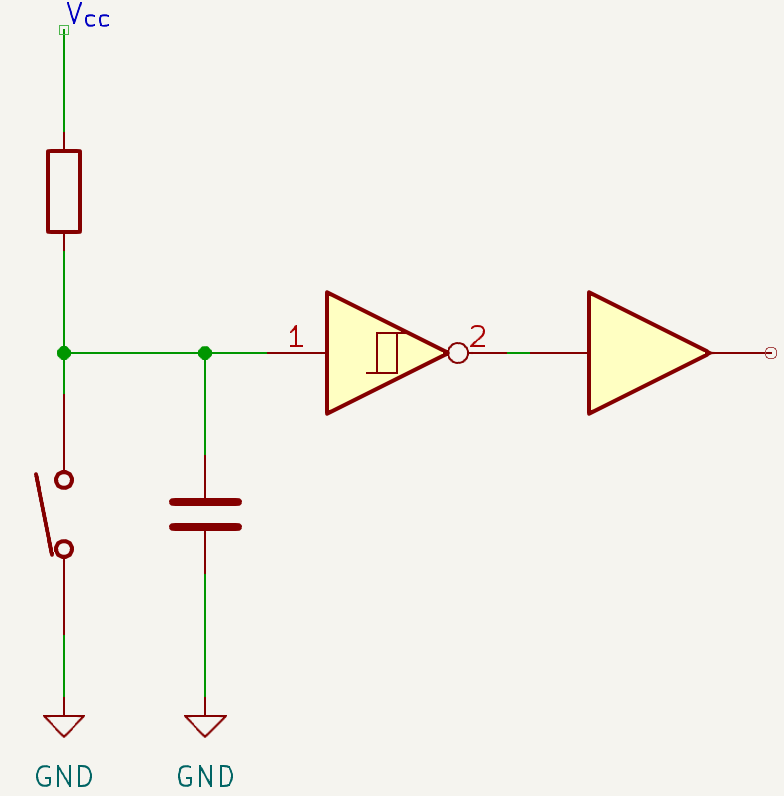
\includegraphics[width=0.6\textwidth]{apply/switch_debounce_schmitt.png}
%     \caption{シュミットトリガ回路を組み合わせたチャタリング防止回路の例}
%     \label{fig:switch_debounce_schmitt}
% \end{figure}
% \newpage

\section{未使用ピンの処理}
論理回路には未使用の入出力ピンが存在する場合がある。
例えば、74HC00は4つのNAND回路を1つのICに内蔵しているが、1つだけNAND回路を使用する場合、残りの3つのNAND回路の入力ピンは未使用となる。
このような未使用の入出力ピンをそのままにしておくと、心理的に不安である。

これらの処理方法を説明する。

未使用の入力ピンは、プルアップ抵抗またはプルダウン抵抗を用いて、論理回路の入力が浮遊状態にならないようにしておけば安心である。
プルアップかプルダウンのどちらを用いるかであるが、出力がLowになるように選ぶとよいとされているが、めんどくさいなら全部プルダウンでよい。

未使用の出力ピンは、基本オープンで大丈夫だが、
オープンコレクタ出力の場合だけは例外で、プルアップかプルダウンをしておく必要がある。
プルアップかプルダウンのどちらを用いるかであるが、消費電力を下げるほうを選ぶとよいとされている。

%論理回路の入出力方法
\chapter{おわりに}

この本を手に取って下さり、ありがとうございました。
今回は初のサークル参加で、時間もなく、少し説明が雑な部分が多くなってしまった気もしますが、論理回路に少しでも興味をもらえれば幸いです。
本書では論理回路の仕組みを中心に話をしてきましたが、割愛した部分も多々あります。今後サークルとしてまた本を出す際には今回端折ってしまった所も説明できたらいいと思っています。
今後も電子回路やロボコン関する本を出していく予定なので、応援してもらえると嬉しいです。

by \quad Ari3
\\
\\

私はもともとコミケなど名前しか知らない状態で、全く関係ない人生を送っていたのですが、Ari3に無理矢理巻き込まれていつの間にか本を書くことになってしまいました。
大学では電気電子工学を専攻しているため、論理回路の理解自体はそこまで難しくなかったのですが、文章にするのは非常に難しく、特に図の作成には苦労しました。
また、Ari3に本を書けと言われたときはすでに12月で、非常にタイトなスケジュールであったため、書きたいこともすべて書ききれず、説明も雑になってしまった部分も多々あるかと思います。
しかし、論理回路の基礎を理解する上で最低限必要なことは盛り込めたと思うので、論理回路に興味を持ってもらえれば幸いです。
来年はより深堀した内容の本を書けたらいいなと思っています。

by \quad El Presidente


\section*{参考文献}
\begin{itemize}
    \item 『ディジタル回路』、斉藤 忠夫、株式会社コロナ社、昭和57年
    \item 『ディジタル回路』、五島 正裕、株式会社数理工学社、2007年
    \item 『ディジタル電子回路』、木村 誠聡、株式会社数理工学社、2012年
\end{itemize}

\newpage
\thispagestyle{empty}

\vspace*{\fill}

\vspace{15em}

\noindent\rule{\textwidth}{0.4pt}

\vspace{1em}

\begin{center}
{\bfseries 理解れ! 論理回路入門}
\end{center}

\vspace{1em}

\noindent
\begin{tabular}{@{}ll@{}}

著者 & Ari3 \quad \& \quad El Presidente \\
サークル & ありのす工房 \\ 
発行日 & 2025年12月31日 初版\\
印刷所 & ペンタロー\\
組版 & \LaTeX \\
連絡先 & chaume.yu@gmail.com\\
twitter &  @early72412338
\end{tabular}

\vspace{1em}

\noindent\rule{\textwidth}{0.4pt}

%おわりに



\end{document}
